%laden der Präambel mit Latexbefehlen/-klassen
%Dokumentklasse und Spracheinstellung
%\documentclass[12pt,oneside,paper=A4,DIV=15,BCOR=0mm,abstract=true,headsepline,headings=normal]{scrreprt}
\documentclass[12pt,twoside,paper=A4,DIV=15,BCOR=22mm,abstract=true,headsepline,headings=normal,parskip=half,ngerman]{scrreprt}
\usepackage{scrhack}
\usepackage[utf8]{inputenc}
\usepackage[T1]{fontenc} % wichtig für Trennung von Wörtern mit Umlauten
\usepackage[ngerman]{babel}

%Schriftart
\usepackage{libertine}
\usepackage{libertinust1math}
\usepackage{csquotes} % for german quotation

%Mathe, Symbole, Einheitendarstellung, Chemie
\usepackage{amsmath}
\usepackage{amsxtra}
\usepackage{eurosym}
\usepackage{siunitx}  
\sisetup{locale=DE}
\usepackage[version=4]{mhchem}
%\usepackage{units}
%\usepackage{cancel}

\usepackage[auto]{microtype}
\clubpenalty = 10000
\widowpenalty = 10000
\displaywidowpenalty = 10000

%Einbindung von Bildern, Tabellen, pdf-Seiten, Quellcode
\usepackage{graphicx}
\usepackage{multirow,multicol,booktabs,makecell}
\usepackage{threeparttable}
\usepackage{longtable}
\usepackage{rotating}
\usepackage{ltablex}
\usepackage{subfig}
\captionsetup[subtable]{position=top}
\usepackage[table]{xcolor}
\usepackage{pdfpages}
\usepackage{listings}
\usepackage{wrapfig}
\graphicspath{{images/}}	% define where to look for images

%Farben


%Darstellung von URL
\usepackage{url}
\urlstyle{same}

%Fussnoten, auch für Tabellen
\usepackage{footnote}
\makesavenoteenv{tabular} 

%Pakete für Kontrolle und Review
\usepackage{todonotes}
\usepackage{blindtext}

%Darstellung der Literaturangaben
\usepackage[
backend=biber,
style=numeric,
citestyle=numeric-comp,
maxbibnames=2,
firstinits=true 
]{biblatex}
\renewcommand*{\labelnamepunct}{\addcolon\addspace}
%Speicherort der Literaturangaben (*.bib Datei)
\bibliography{literature/literaturdatenbank}
% !! Note: Citvi darf keinen Citation Key erzeugen! Nur Bibtex key. Sonst wird 
% "shorthand"-field in bib-file eingefügt. Das überschreibt Zitationsnummer!!!

%Fussnoten
%Markierung in der Fußnote selbst weder hochgestellt noch kleiner gesetzt
%\deffootnote{1em}{1em}{\thefootnotemark\ }
%linksbündige Fußnotenmarkierungen
\deffootnote{1.5em}{1em}{%
	\makebox[1.5em][l]{\thefootnotemark}%
}
\interfootnotelinepenalty=10000 %Fussnoten nicht umbrechen

%Gestaltung der Bildunterschrift und Tabellenüberschirften sowieTitelseitenangaben
\addtokomafont{caption}{\small}
\setkomafont{captionlabel}{\sffamily\bfseries}
\setkomafont{author}{\large}
\setkomafont{date}{\large}
\setkomafont{publishers}{\large}

\renewcaptionname{ngerman}{\figurename}{Abb.}
\renewcaptionname{ngerman}{\tablename}{Tab.} 

%Tabellenumgebungen mit Schriftgröße 10 und 7
\usepackage{tabularx}
\newcolumntype{g}{>{\columncolor{lightgray}}l} %grau hinterlegte Spalte; zentriert
\newcolumntype{L}{>{\raggedright\arraybackslash}X}

% \newenvironment{tabular10}{%
% 	\fontsize{10}{12}\selectfont\tabular
% }{%
% 	\endtabular
% }

% \newenvironment{tabular7}{%
% 	\fontsize{7}{12}\selectfont\tabular
% }{%
% 	\endtabular
% }

% Silbentrennungen


%Verweise und Refernezen, pdf-Eisntellungen
%Angaben aktualisieren! (Für korrekte PDF-Meta-Daten)
\usepackage[
pdftitle={Ausarbeitung eines Use-Cases zur vorrausschauenden Wartung von Zugtüren},
pdfsubject={Masterthesis},
pdfauthor={Daniel Mansfeldt},
pdfkeywords={Predictive Maintenance, PdM, Train},  
%Links nicht einrahmen
hidelinks
]{hyperref}
\usepackage{cleveref}

\begin{document}
%globale Einstellung für Quellcodedarstellung mit listings
%\lstset{basicstyle=\scriptsize\ttfamily,language={[LaTeX]TeX}}


% 							Frontmatter
%================================================================
\begin{titlepage}
	\renewcommand*{\thepage}{Titel}	%nötig damit hyperref die titelseite nicht mit 1 oder röm 1 verwechselt
	\centering
	%{ \LARGE \bfseries Fachhochschule Kiel}
	
	%{\Large University of Applied Siences}
	\begin{figure}
		\centering
		
\includegraphics[keepaspectratio=true,scale=1.5]{FH_Kiel_Logo_deut_rgb.jpg}
	\end{figure}
	
	
	\vspace{2cm}
	{\bfseries \LARGE Masterarbeit}\\
	\bigskip
	zum Erwerb des akademischen	Grades Master of Engineering
	
	\vspace{1cm}
	{\LARGE \bfseries
		\rule{\linewidth}{1pt}\\	% \\ generiert einen Zeilenumbruch, wie eine Leerzeile.
		%usepackage{csquotes} nötig für \enquote{text}
		Ausarbeitung eines Use-Cases zur vorrausschauenden Wartung von Zugtüren\\
		\rule{\linewidth}{1pt}
	}
	
	\vspace{1cm}
	vorgelegt von\\
	\bigskip
	Daniel Mansfeldt
	
	
	\vspace{3cm}
%	\raggedright{
	\begin{tabular}{ll}
		Fachbereich: & Maschinenwesen\\
		Studiengang: & Master Maschinenbau\\
		Matrikelnummer: & 926843\\
		&\\
		Erstprüfer: & Herr Prof. Dr.-Ing. Daniel Böhnke\\
		Zweitprüfer: & Herr Prof. Dr.-Ing. Henning Strauß\\
		&\\
		Datum: & \today
	\end{tabular}
%	}
\end{titlepage}
\cleardoublepage

\pagenumbering{roman}
% \begin{center}
% 	\textbf{Sperrvermerk}
% \end{center}
% \raggedright
% Die vorgelegte Masterarbeit mit dem Titel:

% „TITEL EINFÜGEN“

% beinhaltet vertrauliche und interne Daten der Forschungseinrichtung:

% Institut für fluidtechnische Antriebe und Systeme der RWTH Aachen

% Campus Boulevard 30 D-52074 Aachen

% \textbf{Die Einsicht in die Bachelorarbeit ist Unbefugten nicht gestattet. Ausgenommen hiervon sind die Gutachter sowie berechtigte Mitglieder des Prüfungsausschusses. Die Vervielfältigung und Veröffentlichung der Bachelorarbeit – auch auszugsweise – ist grundsätzlich nicht erlaubt.}

% Eine Ausnahme von dieser Regelung bedarf einer Erlaubnis der oben genannten Forschungseinrichtung.

% \clearpage

%======Eigesstattliche Versicherung==============

\begin{center}
	\textbf{Eidesstattliche Versicherung}
\end{center}
\vspace{2cm}

\parbox{7cm}{\rule{7cm}{1pt}\\Name, Vorname}
\hfill 
\parbox{7cm}{\rule{7cm}{1pt}\\Matrikelnummer}
\vspace{1cm}

Ich versichere hiermit an Eides Statt, dass ich die vorliegende Masterarbeit mit dem Titel

\glqq Ausarbeitung eines Use-Cases zur vorrausschauenden Wartung von Zugtüren\grqq

selbständig und ohne unzulässige fremde Hilfe erbracht habe. Ich habe keine anderen als
die angegebenen Quellen und Hilfsmittel benutzt. Für den Fall, dass die Arbeit zusätzlich auf
einem Datenträger eingereicht wird, erkläre ich, dass die schriftliche und die elektronische
Form vollständig übereinstimmen. Die Arbeit hat in gleicher oder ähnlicher Form noch keiner
Prüfungsbehörde vorgelegen.

\vspace{2cm}
\parbox{7cm}{\rule{7cm}{1pt}\\Ort, Datum}
\hfill 
\parbox{7cm}{\rule{7cm}{1pt}\\Unterschrift}
\clearpage
%------------------Deutsch------------------
% =>
\begin{center}
	\textbf{Kurzfassung}
\end{center}
\raggedright
Die vorausschauende Instandhaltung verspricht deutliche Verbesserungen bei der Wartung, Inspektion, Instandsetzung und Verbesserung von Systemen und Anlagen gegenüber der heute zu tage üblichen präventiven Instandhaltung. Insbesondere im Kontext der Industrie~\num{4.0} sind die Erwartungen an die Auswertung großer Datenmengen groß.

Trotz der großen Potentiale der vorausschauenden Instandhaltung sind bis lang relativ wenige Anwendungsfälle erschlossen. In der Regel ist eine präzise Abschätzung nötig ob sich die Implementierung eines PDM-Usecases lohnt.

Wenn auch nicht zwingend erforderlich, so kommen doch häufig maschinelle Lernalgorthmen für PDM-Usecases zum Einsatz. Diese sind für eine sinnvolle Umsetzung sorgfälltig auszuwählen und an die gegebenen Umstände anzupassen.

In dieser Arbeit soll ein potentieller PDM-Usecase für die Instandhaltung einer Zugtür erdacht werden; genauer für die Wartung der Umlenkrollen eines Bautenzuges. Es wird begründet welche Messwerte benötigt werden, um den Zustand der Umlenkrollen zu bestimmen, um daraus Maßnahmen für die Instandhaltung ableiten zu können. Mit den Daten wird anschließend eine Auswahl maschineller Lernmodel trainiert und das am besten für den Usecase geeignete Model bestimmt. Dazu wird sowohl auf die Eigenschaften der Modelle eingegangen, wie auch die Erfolgskriterien des Usecases berücksichtigt und die Ergebnisse in diesem Kontext diskutiert. Schlussendlich kann so eine Einschätzung abgegeben werden, ob der vorgeschlagene Usecase mit dem entwickelten Model eine brauchbare Anwendung von PDM darstellt.

Der Usecase wird außerdem im Kontext der aktuellen Bahntechnik diskuiert.
% <=
%-------------------------------------------
\clearpage
%------------------English------------------
% =>
\begin{center}
	\textbf{Abstract}
\end{center}
\raggedright
english
% <=
%-------------------------------------------
\clearpage

\cleardoubleemptypage

%Inhaltsverzeichnis
%Es werden nur Kapitel und Abschnitte angezeigt. Unterabschnitte (/subsection) nicht mehr. Sonst tocdepth höher einstellen.
\setcounter{tocdepth}{1}
\tableofcontents
\cleardoubleemptypage
%================================================================


% 							Mainmatter
%================================================================
%Seitennummerierung zurücksetzen und arabisch
\pagestyle{headings}
\pagenumbering{arabic}
\setcounter{page}{1}

%Beginn der Kapitel
\chapter{Einleitung}
\label{ch:einleitung}

\section{Problemstellung}
\label{sec:motivation}
WAS SOLL IN DER MASTERARBEIT BEHANDELT WERDEN?

Die vorausschauende Instandhaltung (engl. \textit{Predictive Maintenance}; kurz \textit{PdM}) bietet im Vergleich mit anderen Instandhaltungsstrategien großes Verbesserungspotential. Insbesondere im Zusammenhang mit der Industrie~{4.0} hat PdM in den letzten Jahren viel Aufmerksamkeit gewonnen. PdM rückt für zunehmend mehr Anwendungen in den Fokus, ist heute aber nach wie vor nur in wenigen Fällen zu finden. 

Ein Grund dafür warum PdM weniger verbreitet ist als z.B. präventive Methoden ist zum einen der hohe Investitionsaufwand und zum anderen die Tatsache, dass in vielen Bereichen mögliche Anwendungsfälle nicht bekannt sind. Zwar ist es denkbar, dass für den speziellen Fall eine andere Herangehensweise die Bessere ist, jedoch selbst um dies festhalten zu können, muss das Potential für die jeweilige Anwendung analysiert werden. 

Im Kern handelt es sich bei der Machbarkeitsstudie eines neuen PdM-Usecases um ein Data-Mining-Problem; also um die Gewinnung von Informationen anhand von Daten. Entsprechend kann der \textit{Cross-industry standard process for data mining}; kurz CRISP-DM; angewendet werden.

Grundsätzlich bedarf es einer umfassenden Analyse eines neuen PdM-Usecases ehe dieser Umgesetzt werden sollte.

Die vorausschauende Instandhaltung bietet im Vergleich zur präventativen Instandhaltung das Potentiale der Senkung der Instandhaltungskosten und einen darüber hinausgehenden Informationsgewinn der auch für Prozesssteuerung und Verbesserungen genutzt werden kann. Dies ist aber nur unter bestimmten Voraussetzungen der Fall, welche sich dazu vom betrachteten Fall abhängen.

Um eine Einschätzung über das Potential eines bestimmten Anwendungsfall abgeben zu können, ist es notwendig diesen so weit zu erarbeiteten, dass ein Vergleich mit dem zu ersetzenden Verfahren sinnvoll durchgeführt werden kann.

Für die vorausschauende Wartung sind Vorhersagemodelle nötig. Deren Qualität ist einer der wichtigste Faktor für den Nutzen des gesamten Anwendungsfalls. Ist beispielsweise die Verhinderung von Ausfällen und eine besserte Ausnutzung der Bauteillebensdauer das Ziel, so muss das Model Vorhersagen treffen die zu einem gewissen Maß zutreffend sind, um einem anderen Verfahren gegenüber bevorzugt werden zu können.

Soll ein maschinelles Lernmodel verwendet werden, um Vorhersagen für einen Anwendungsfall der vorausschauenden Wartung abzugeben, so muss ein solches Model zunächst modelliert und bewertet werden.


Mit dem Aufschwung der Industrie 4.0 und der damit einhergehenden stetig größer weredenden Menge verfügbarer Daten, rückt PDM jedoch aus Nischenanwendungen aktuell weiter in den Fokus von Anlagenbetreidenden. Schließlich bieten sich durch eine große Menge Daten neue Möglichkeiten. Nicht nur können bestehende Anwendungen mit größerer Präzision ausgeführt werden; es ergeben sich auch grundlegend neue Anwendungsmöglichkeiten. \todo{Beispiel}

PDM ist in vielen technischen Bereichen insbesondere deshalb interessant, weil  dadurch nach Hölzel folgende Potentiale erschlossen werden können \todo{Verweis auf Hölzel S.31}. Diese sind in abgrenzung zur präventiven Instandhaltung zu sehen:
\begin{itemize}
	\item Bedarfsgerechte Ersatzteilbereitstellung
	\item Instandhaltungsmaßnahmen können zum optimalen Zeitpunkt durchgeführt werden
	\item Verlängerung der anlagen- und Bauteillebensdauer
	\item Reduzierte Stillstandzeiten
	\item Reduzierte Instandhaltungskosten
	\item Verbesserung der Anlagenzuverlässigkeit
\end{itemize}

Auch für die Instandhaltung von Schienenfahrzeugen erscheinen PDM-Anwendungen interessant. Neben den oben genannten Punkten scheint sich durch die Verringerung von Ausfällen auch Imageschaden abzuwenden. Dieser Entsteht, wenn  der Ausfall einer Anlage sich direkt auf den Kunden auswirkt; in diesem Fall der Fahrgast.

Ein für Fahrgäste zu beobachtender Fall sind Türstörungen. In der Regel äußern sich diese darin, dass die Zugtür nicht mehr entsprechend der Sicherheitsanforderungen nutzbar sind. In den meisten Fällen genügt es jedoch die Tür außer Betrieb zusetzen und um so die Sperrung eines Waggons oder gar den Ausfall einer ganzen Fahrt zu verhindern. Dennoch ist der Ausfall einer Zugtür für den Kunden direkt ersichtlich und führt damit zu einem Imageschaden. Aus diesem Grund erscheint der Einsatz vorausschauender Wartung auch hier sinnvoll. Auch aus technisch wirtschaftlicher Sicht.

Die Fragestellung die bei der Umsetzung aller PDM-Anwendungen zunächst geklärt werden muss ist, ob das entwickelte Modell zur Vorhersage ausreichend präzise Vorhersagen trifft. Insbesondere entscheidend ist dabei der vergleich mit der gegenwärtigen Instandhaltungsstrategie.

In jedem Fall muss die Frage geklärt werden, ob sich die Umstellung auf ein vorrauschauendes Instandhaltungsprogramm lohnt. Ein umfangreiche Analyse der zu erwartenden Kosten stellt die Grundlage zur Beantwortung dieser Frage dar. Das Vorhersagemodel, auf dem der Anwendungsfall basiert, stellt die wichtigste Grundlage zur Kostenanalyse dar. Ohne eine zuverlässige Einschätzung über die Treffsicherheit der Vorhersagen, kann kein Kostenvergleich zu einem anderen Verfahren erstellt werden. Die Entwicklung eines Vorhersagemodels stellt deswegen eine entscheidende Grundlage dar. 

% \begin{figure}[ht]
% 	\centering
% 	
\includegraphics[scale=0.4]{FH_Kiel_Logo_deut_rgb.jpg}
% 	\caption{Logo}
% 	\label{fig:fhlogo}
% \end{figure}

\section{Ziel der Arbeit}
\label{sec:ziel}
In dieser Arbeit soll eine erste Iteration des CRISP-DM-Models durchlaufen werden.

F: WAS SOLL ERARBEITET WERDEN? WELCHE ERKENNTNISSE SOLLEN GEWONNEN WERDEN?
A: DAS KONZEPT DES Usecases SOLL BESCHRIEBEN WERDEN

Zunächst soll eine neuer PdM-Usecase beschrieben werden, der auf die Erkennung von beschädigten Bauteilen abzielt. Dabei soll lediglich eine Klassifikation mit zwei Kategorien; \enquote{intakt} und \enquote{beschädigt} möglich sein. In diesem Zusammenhang sollen auch Kriterien beleuchtet werden, an denen eine erfolgreiche Umsetzung des Usecases gemessen werden kann.

F: WAS SOLL ERARBEITET WERDEN? WELCHE ERKENNTNISSE SOLLEN GEWONNEN WERDEN?
A: EIN VERSUCH ZUR DATENAUFNAHME SOLL DURCHGEFÜHRT WERDEN

Um eine Klassifikationsmodel entwickeln zu können, mit dem der Usecase Umgesetzt werden kann, wird ein Datensatz aufgenommen. Dazu werden an der Türschließanlage Messungen durchgeführt. Für intakte und beschädigte Umlenkrollen wird eine Auswahl an Messwerten aufgenommen. 

F: WAS SOLL ERARBEITET WERDEN? WELCHE ERKENNTNISSE SOLLEN GEWONNEN WERDEN?
A: DIE BEDEUTUNG DER DATEN FÜR DEN USECASE SOLLEN BESTIMMT WERDEN
A: WIE MUSS DER DATENSATZ AUFBEREITET WERDEN?

Im Zuge des \textit{Dataunderstanding} wird die Bedeutung der Daten für den Usecase diskutiert. Dabei wird außerdem ein Datensatz erarbeitet, der den rohen Datensatz beschreibend zusammenfasst. Ziel ist dabei den Informationsgehalt der Daten zu bündeln und so die Verallgemeinerungsleistung der Modelle zu fördern.

F: WAS SOLL ERARBEITET WERDEN? WELCHE ERKENNTNISSE SOLLEN GEWONNEN WERDEN?
A: MEHRERE MODELLE SOLLEN MODELLIERT WERDEN

Um ein Model zu bestimmen, das die besten Vorhersagen über den Zustand der Umlenkrollen liefert, wird zunächst eine Vorauswahl infrage kommender Modeltypen durchgeführt. Anschließend werden Modelle der in frage kommenden Typen erstellt. Dabei wird für jedes Model eine Parameterstudie durchgeführt.

F: WAS SOLL ERARBEITET WERDEN? WELCHE ERKENNTNISSE SOLLEN GEWONNEN WERDEN?
A: DAS BESTE FÜR DEN USECASE SOLL BESTIMMT WERDEN

Nach der Modelierung erfolgt eine Bewertung der Modelle. Anhand ausgewählter Kriterien, die für den Usecaes relevant sind, wird das am besten geeignete Model bestimmt.

F: WAS SOLL ERARBEITET WERDEN? WELCHE ERKENNTNISSE SOLLEN GEWONNEN WERDEN?
A: ES SOLL EIN AUSBLICK GEGEBEN WERDEN WIE DER USECASE ZU ANWENDUNGSREIFE WEITER ENTWICKELT WERDEN KANN

Abschließend soll ein Ausblick gegeben werden, der mögliche nachfolgende Schritte beleuchtet, um den Anwendungsfall praxistauglich zu gestalten, sollte ein geeignete Vorhersagemodel entwickelt werden können.



















Der System von Interesse in dieser Arbeit ist eine Türschließanlage. Diese findet in Intercity-Züge der Deutschen Bahn Anwendung. Für ausgewählte Komponenten der Anlage wird ein Anwendungsfall zur vorausschauenden Wartung der Komponenten erdacht. Dabei wird das Ziel verfolgt den Zustand einer Komponenten anhand von Sensordaten klassifizieren zu können. 

Es soll ein PdM-Usecase zu einer Komponente der Türschließanlage erdacht werden. Den Kern dieser Arbeit stellt darauf aufbauend die Entwicklung eines maschinellen Lernmodels dar, das eine Klassifikation einer Komponente vornehmen kann. Unterschieden werden soll dabei zwischen intakte und beschädigten Bauteilen. Bei der Entwicklung des Models sollen sowohl Erfolgskriterien für den potentiellen Anwendungsfall, wie auch Eigenschaften der betrachteten Modeltypen berücksichtigt werden. Aus einer Auswahl an Modellen soll das beste für den gegebenen Anwendungsfall bestimmt werden.

Das Modell soll in der Lage sein Beschädigungen einer Umlenkrolle zu erkennen. Die Umlenkrolle mit dem ein simulierter Schadenfall vorhergesagt werden könnte. Die Arbeit ist dabei vor der Vision angesiedelt maschinelle Lernverfahren für die vorausschauende Instandhaltung einzusetzten. Entsprechend sollen die Ergebnisse der Modelentwicklung vor diesem Hintergrund beleuchtet werden.

\section{Vorgehensweise}
\label{sec:vorgehensweise}
WELCHE SCHRITTE WERDEN DURCHLAUFEN UM DIE ANGESTREBTEN ERGEBNISSE ZU ERHALTEN?
(LÄSST SICH NACH KAPITELN ORDNEN)

In den Kapiteln 2 bis 4 wird der Stand der Technik der Elemente beschrieben, die für den Inhalt der Arbeit von Bedeutung sind. \cref{ch:vorausschauende instandhaltung} befasst sich mit den grundlegend mit der vorausschauenden Instandhaltung und diskutiert dessen Potentiale und Voraussetzungen.

In \cref{ch:maschinelles lernen} werden zunächst Kernpunkte von maschinellem Lernen erörtert, ehe auf die Grundlagen der Lernmodelle eingegangen wird, die im weiteren Verlauf dieser Arbeit verwendet werden. Für die einzelnen Modelle werden u.a. Funktionsweise, Parametereinstellungen, Vor- und Nachteile, sowie die Eignung für den in \cref{ch:usecase} dargestellten Anwendungsfall besprochen. 

\cref{ch:usecase} stellt den neu erdachten PDM-Usecase vor. Dabei wird an den entsprechenden Stellen auf die Inhalte aus \cref{ch:vorausschauende instandhaltung} verwiesen und ein Beispielszenoario beschrieben, wie die Anwendung des Usecases aussehen könnte. Um den Usecase in den Kontext der praktischen Bahntechnik zu setzen, werden die Inhalte zweier Interviews mit Bahnsachverständigen rekapituliert. In Zuge dessen wird auch der reale Bedarf des vorgeschlagenen Usecases diskutiert. Die Darstellung des Usecases schließt mit einer Aufführung der Erfolgskriterien des Usecases.

In \cref{ch:methodik} wird die Methodik beschrieben mit der der Usecase exemplarisch untersucht wurde. Es wird der Versuchaufbau beschrieben, eine Einschätzung über den Datensatz abgegeben und eine begründete Vorauswahl maschineller Lernmodelle getroffen (vgl. \cref{ch:maschinelles lernen}). In \cref{sec:bewertungskriterien} werden die Erfolgskriterien des Usecases aus \cref{ch:usecase} aufgegriffen, um die zu erstellenden Modelle daran bewerten zu können. In \cref{sec:praeferenzfunktion} wird damit eine Präferenzfunktion zur Beurteilung der Modelle erstellt.

In \cref{ch:modelierung} erfolgt die Erstellung der maschinellen Lernmodelle anhand des aufgenommen Datensatzes. Um möglichst gute Modelqualitäten zu erreichen wird während des Trainieren der Modelle eine Parameterstudie durchgeführt.

In \cref{ch:modelbewertung} wird die Eignung der trainierten Modelle für den Usecase dargestellt und diskutiert. Es wird eine Einschätzung über die Qualität der Modelle abgegeben und anhand der Präferenzfunktion das Model bestimmt welches am besten für den Usecase geeignet ist.

\cref{ch:fazit} fasst die Ergebnisse der Arbeit zusammen und gibt einen Ausblick über Verbesserungsmöglichkeiten in Bezug auf den Usecase an sich und die erarbeiteten Ergebnisse.\cleardoublepage
% \chapter{Instandhaltungsstrategien}
\label{ch:instandhaltungsstrategien}
Die Norm DIN~31051~\cite{DIN.2019} definiert die \textit{Instandhaltung} allgemein als \enquote{Kombination aller technischen und administrativen Maßnahmen sowie Maßnahmen des Managements während des Lebenszyklus [\dots] eines Objekts [\dots], die den Erhalt oder der Wiederherstellung ihres funktionsfähigen Zustands dient, sodass es die geforderte Funktion [\dots] erfüllen kann}. Darüber hinaus enthält die Normschrift Definitionen für die folgenden Unterkategorien der Instandhaltung

\begin{table}[ht]
	\centering
	\begin{tabularx}{\textwidth}{ | l | X |}
		\hline
        \rowcolor{lightgray}
        Unterkategorie & Definition\\
        \hline
        Wartung & \enquote{Maßnahmen zur Verzögerung des Abbaus des vorhandenen \textit{Abnutzungsvorrats}.}\\
        \hline
        Inspektion & \enquote{Prüfung auf Konformität der maßgeblichen Merkmale eines \textit{Objekts […]}, durch Messung, Beobachtung oder Funktionsprüfung}\\
        \hline
        Instandsetzung & \enquote{physische Maßnahme, die ausgeführt wird, um die Funktion eines fehlerhaften \textit{Objekts […] }wiederherzustellen.}\\
        \hline
        Verbesserung & \enquote{Kombination aller technischen und administrativen Maßnahmen sowie Maßnahmen des Managements zur Steigerung der immanenten Zuverlässigkeit und/oder Instandhaltbarkeit und/oder Sicherheit eines \textit{Objekts […]}, ohne seine ursprüngliche Funktion zu ändern.}\\
        \hline
	\end{tabularx}
	\caption{Definitionen von Unterkategorien der Instandhaltung nach DIN~{31051}~\cite{DIN.2019}}%muss unten sein, sonst caption über Tab
	\label{tab:definition_unterkategorien_instandhaltung}	%zum referenzieren
\end{table}

Es gibt unterschiedliche Herangehensweisen bzw. Philosophien nach denen Instandhaltung umgesetzt werden kann; nach DIN~13306~\cite{DIN.2018} werden sie von hier an als \textit{Instandhaltungsstrategien} bezeichnet. In der Literatur herrscht keine Einheitlichkeit bei der Einordnung oder Benennung der Instandhaltungsstrategien. Das U.S. Department of Defense~\cite[S.~16]{U.S.DepartmentofDefense.2008} unterscheidet drei Strategien, die im Rahmen dieser Arbeit verwendet werden. Unten sind die drei Instandhaltungsstrategien zusammen mit ihrer englischen Bezeichnung und einer Abkürzung aufgeführt.

\begin{itemize}
    \item Korrektive Instandhaltung - Corrective Maintenance (CM)
    \item Präventive Instandhaltung - Preventive Maintenance (PM)
    \item Prädiktive Instandhaltung - Predictive Maintenance (PdM)
\end{itemize}

Die drei Instandhaltungsstrategien unterscheiden sich grundlegender Weise dadurch, wie Instandhaltungsmaßnahmen ausgelöst werden. Pauschal kann keine Aussage darüber getroffen werden, welche der drei Instandhaltungsstrategien für einen gegebenen Anwendungsfall am besten geeignet ist. Neben wirtschaftlichen Aspekten müssen ggf. auch sicherheitstechnische, ethische und umweltrelevante Aspekte berücksichtigt werden.
%===============================================================================
\section{Korrektive Instandhaltung}
\label{sec:korrektive_instandhaltung}
Im Falle der rein korrektiven Instandhaltung wird eine Instandhaltungsmaßnahme erst dann initiiert, wenn ein System seine Funktion nicht mehr erfüllen kann. Selbst Wartungsmaßnahmen, wie der regelmäßige Austausch von Schmierstoffen, werden nicht durchgeführt solange es nicht zur Behebung des Funktionsausfalls nötig ist.~\cite[S.~2]{Mobley.2002}

Die korrektive Instandhaltung ist die teuerste unter den drei genannten Strategien. Durchschnittlich fällt sie dreimal so teuer aus, wie eine präventive Instandhaltung der gleichen Anlage. Ursachen dafür sind u.a. hohe Kosten für kurzfristige Beschaffung bzw. Lagerung von Ersatzteilen, vergleichweise lange Ausfallzeiten und hohe Arbeitskosten.~\cite[S.~3]{Mobley.2002}

In der Praxis wird selten eine rein korrektive Instandhaltungsstrategie verfolgt. Selbst in Fällen in denen es wirtschaftlich sinnvoll ist, Instandsetzungsmaßnahmen erst dann einzuleiten, wenn eine Störung aufgetreten ist, werden üblicherweise trotzdem grundlegende Wartungsarbeiten durchgeführt. Diese sind der präventiven Instandhaltung zuzuordnen.~\cite[S.~2]{Mobley.2002}
%===============================================================================
\section{Präventive Instandhaltung}
\label{sec:praeventive_instandhaltung}
Im Sinne einer präventiven Instandhaltung werden vorbeugende Maßnahmen getroffen. Wartungs-, Inspektions-, und Verbesserungsarbeiten verfolgen das Ziel Störungen zu verhindern. Dies geschieht beispielsweise durch den regelmäßigen Austausch verschleißender Komponenten und Betriebstoffe oder konstruktive Änderungen. Instandsetzungsmaßnahmen sind nur nötige, wenn es trotz der vorbeugenden Maßnahmen zu einer Störung gekommen ist.

Das Intervall, in dem vorbeugende Arbeiten ausgeführt werden, ist stets von Abschätzungen und Erfahrungswerten über die Zustandsänderung des Systems abhängig. Dabei handelt es sich meist um statischtische Betrachtungen. Der Zeitpunkt eines Komponentenausfalls oder anderweitiger Störung kann somit nicht exakt vorhergesagt werden. Um Störungen mit ausreichender Wahrscheinlichkeit verhindern zu können, wird z.B. ein Komponentenwechsel vor dem erwarteten Ende dessen Lebensdauer angesetzt. Hölzel fasst die Folgen wie folgt zusammen: \enquote{Der routinemäßige Austausch von noch funktionsfähigen Komponenten führt zu einer Verschwendung von Ressourcen}~\cite[S.~29]{Holzel.2019}.
%===============================================================================
\section{Prädiktive Instandhaltung}
\label{sec:praediktive_instandhaltung}
Prinzipiell verfolgt auch die vorrauschauende Instandhaltung das Ziel Ausfälle durch präventive Maßnahmen zu verhindern. Im Gegensatz zur rein präventiven Instandhaltung setzt diese Strategie jedoch auf Kenntnis über den aktuellen Zustands einer Anlage oder Komponente voraus. Werden diese Informationen auf bekannte Zusammenhänge projiziert können konkrete Vorhersagen über den zukünftigen Verlauf des Zustandes getroffen werden. Eine Ressourcenverschwendung durch den Austausch funktionsfähiger Komponenten kann so auf ein Minimum reduziert werden, weil beispielsweise der Zeitpunkt des Versagens der Komponente genauer vorhergesagt werden kann.

Voraussetzung für PdM ist es zu einem beliebigen Zeitpunkt den Zustand einer Anlage bestimmen zu können. So können Instandhaltungsmaßnahmen günstiger terminiert werden als dies bei der präventive Instandhaltung möglich ist. Für viele Anwendungsfälle ist dafür eine kontinuierliche, automatisierte und sensorbasierte Überwachung nötig. Manuelle Inspektionen sind in einem solchen Umfang nur in seltenen Fällen wirtschaftlich tragbar. Die kontinuierliche Überwachung von Systemen ist unter dem englischen Begriff \textit{Condition Monitoring} bekannt.

Durch fortlaufende Kenntnis um den aktuellen Zustand einer Anlage oder Komponente, sowie dessen voraussichtlich weiterer Verlauf, ergibt sich eine Reihe von Kostenvorteilen gegenüber den anderen beiden Instandhaltungsstrategien. Besteht beispielsweise Kenntnis über einen schmalen Zeitbereich in dem eine Komponente ausfallen wird, können Ersatzteile mit ausreichendem Planungsvorsprung beschafft werden. Eine kostenintensive Lagerung oder kurzfristige Anfertigung der Ersatzteile ist nicht notwendig. Über die Instandhaltung hinaus können außerdem die gewonnen Informationen für die Prozesssteuerung genutzt werden. Aus einer Zustandsänderung von Komponenten folgt zwangsläufig eine Änderung der Prozessparameter. Mit der Kenntnis, wie sich ein gewisser Zustand einer Komponenten auf den Gesamtprozess auswirkt, können entsprechende Anpassungen der Prozesseinstellungen vorgenommen werden. PdM lässt sich für die Prozesssteuerung und folglich auch für die Qualitätssicherung verwenden.

Zu den Nachteilen von PdM gehört der große Investitionsaufwand. Erstens ist eine umfangreiche Analyse notwendig, um den Mehrwert einer PdM-Anwendung festzustellen; sofern dieser existiert. Zweitens bedeutet die Einführung eines Condition-Monitoring-Systems einen nicht vernachlässigbaren Kostenaufwand. Drittens sind unter Umständen Fortbildungen der Belegschaft oder der Einkauf von qualifiziertem Personal nötig, um ein PdM-Programm zu betreiben. 
%===============================================================================\cleardoublepage	
% \chapter{Machine Learning}
\label{ch:machine_learning}
F: Was ist maschinelles lernen? welchen Zweck hat es?

Maschinelles Lernen (ML) ist \enquote{ein Forschungsfeld in der Schnittmenge von Statistik, künstlicher Intelligenz und Informatik}~\cite[S.~1]{Muller.2017}. Heute wird ML in vielen kommerziellen Bereichen genutzt; ebenso wie in der datengetriebenen Forschung. Die steigende Komplexität von Problemen hat dazu geführt, dass die individuelle Anfertigung von Programmen zur Lösung einer Problemstellung, häufig nicht mehr praktikabel ist. So muss ein ein Programm bereits für eine kleine Änderung der Problemstellung aufwendig überarbeitet werden oder die Aufgabe an sich übersteigt die Fähigkeit eines Experten, das Problem in seiner vollständigen Komplexität zu erfassen. Müller~\cite{Muller.2017} nennt in diesem Zusammenhang die Entwicklung von Gesichtserkennungssoftware als Beispiel. Er betont, dass aufgrund der grundsätzlich verschiedenen "Wahrnehmung" von Bildern zwischen Menschen und Computern, es für den Menschen unmöglich ist allgemeingültige Regeln zum Erkennen von Gesichtern zu definieren, die eine Software einsetzten könnte. Während Menschen einen optischen Eindruck von der Welt erhalten, sind Computer bei der Interpretation von Bildern auf Farbwerte einzelner Pixel angewiesen; sprich eine konkrete Menge diskreten Zahlenwerte. Die Entwicklung maschineller Lernalgorithmen hat es jedoch möglich gemacht das Erstellen von Entscheidungsmodellen weitgehend zu automatisieren.  

F: welche Unterkategorien gibt es beim machine learning?

Man unterscheidet beim maschinellen Lernen zwischen \textit{überwachten} und \textit{unüberwachten} Lernen. Beim überwachten Lernen werden dem Algorithmus Datenpunkte mit zugehörigem Zielwert übergeben. Im der Algorithmus verallgemeinernde Kriterien bestimmt an denen sich die Datenpunkte dem richtigen Zielwert zuordnen lassen, entsteht ein Model mit dem eine Zuordnung von zuvor unbekannten Datenpunkten getroffen werden kann. Der Zielwert kann dabei ein diskreter Wert (Klassifikation) oder eine kontinuierliche Variable (Regression) sein. Ein Beispiel für eine Klassifikationaufgabe eines überwachten Lernalgorithmus ist die Unterscheidung zwischen normalen Emails und Spam-Emails \cite[S.~2]{Muller.2017}.

Beim unüberwachten Lernen stehen für einen Datensatz keine Informationen über die Zielwerten zur Verfügung. Ziel dieses Ansatzes ist es Cluster in einem gegebenen Datensatz zu finden, um daraus weitere Schlüsse ziehen zu können.

F: Was hat ML mit PdM zutun?

Im Zuge der Digitalisierung von Produktionsprozessen stehen zunehmend größere Datenmengen zur Verfügung. Aus dieser Entwicklung folgt, dass Herausforderungen der Prozessoptimierung vom Datamining- und Machine Learning-Ansätzen profitieren können.~\cite[S.~35]{Schafer.25.09.201927.09.2019}

Die Einführung einer PdM-Anwendung anstelle einer anderen Instandhaltungsstrategie stellt einen Optimierungsprozess dar. Sowohl zur Klärung der Frage, ob die PdM-Anwendung eine Verbesserung darstellt, und für den Gebrauch der Anwendung müssen Modelle entwickelt werden, die die Verarbeitung der Anwendungsdaten ermöglichen. Maschinelle Lernalgorithmen sind dafür nützliche Tools, weil sie diese Prozesse vereinfachen (s.o.).

\section{Machine Learning Algorithmen mit Entscheidungsbäumen}
\label{sec:algorithmen_mit_entscheidungsbaum}
F: Was sind Entscheidungsbäume?

Entscheidungsbäume sind komplexe Entscheidungsstrukturen. \todo{Bild einfügen Entscheidungsbaum} zeigt den prinzipiellen Aufbau eines Entscheidungsbaums.

F: wie FUNKTIONIEREN Entscheidungsbäume?

Ein Datenpunkt wird durch einen Entscheidungsbaum einer Kategorie oder einem Wert zugeordnet. Zunächst wird anhand eines Merkmals eine Entscheidung im Wurzelknoten des Baums getroffen. Je nach Ergebnis wandert der Datenpunkt in einen der darunter liegenden Knoten. Hier wird nun ein anderes Merkmal beurteilt und der Datenpunkt entsprechend dem nächsten Knoten oder -- im letzten Schritt -- einem Blatt zugeordnet. Den Blättern sind die Kategorien oder Werte zugeordnet, welche mit jedem Datenpunkt assoziiert wird, welcher sich in dem Blatt befindet. 

F: wie wird ein Entscheidungsbaum trainiert

Um das Entscheidungskriterium für jeden Knoten zu bestimmen, werden sämtliche möglichen Merkmale überprüft und der Wert bestimmt der den vorhandenen Datensatz am besten den richtigen Zielwerten zuordnen kann. Dies wird für alle Teilungen durch die Knoten wiederholt.~\cite{Muller.2017}

F: wie kann der Aufbau kontrolliert werden

Ohne Beschränkungen würde ein Entscheidungsbaum solange weiter aufgebaut werden bis jedes Blatt nur einen einzelnen Datenpunkt enthält. Ein derart aufgebauter Entscheidungsbaum ist in der Regel ungeeignet, um damit zutreffende Zielwerte für neue Datenpunkte bestimmen zu können. Das Model orientiert sich zu stark an den Merkmalswerten aus dem Trainingsdatensatz und ist daher nicht in der Lage gute verallgemeinernde Entscheidungskriterien zu finden. Man spricht in diesem Zusammenhang von \textit{Overfitting}. Um Overfitting entgegen zu wirken kann beispielsweise die minimale Anzahl der Datenpunkte in einem Blatt limitiert werden oder die Tiefe des Baums und damit die Anzahl der Knoten begrenzt werden.

F: welche Modelle gibt es? welche sind interesant hier?

Es gibt verschiedenen Arten von ML-Modellen, die auf Entscheidungsbäumen basieren. Sie unterscheiden sich sowohl in der Strategie zum Aufbau der Bäume; der Anzahl der Bäume; als auch der Ermittlung des Gesamtergebnisses für einen Datenpunkt. 

Im weiteren Verlauf dieser Arbeit werden drei verschiedene maschinelle Lernalgorithmen angewendet, die auf Entscheidungsbäumen basieren. In den folgenden Abschnitten werden wichtige Eigenschaften dieser Modeltypen beleuchtet. Alle drei Modeltypen sind für die Programmiersprache \textit{Python} in dem Packet \textit{scikit-learn} implementiert.

\subsection{Einfache Entscheidungsbäume}
\label{sec:einfache_entscheidungsbaeume}
F: was ist das?

Der einfachste Modeltyp, der auf Entscheidungsbäumen beruht, ist ein einzelner Entscheidungsbaum. Wie in \cref{sec:algorithmen_mit_entscheidungsbaum} beschrieben, entspricht die Beurteilung eines Datenpunktes der Kategorie des Blatts, das den Datenpunkt beinhaltet.

Ein einzelner Entscheidungsbaum lässt sich praktikabel visualisieren; vorausgesetzt seine Knotenanzahl ist überschaubar. Das Verfahren nach dem der Baum Entscheidungen triff, kann so durch Sachverständige nachvollzogen und beurteilt werden. Dies ist der entscheidende Vorteil gegenüber anderen Modelarten, wie dem Random Forest oder den Gradient Boosted Trees.

Nachteil von Entscheidungsbäumen ist das sie zu Overfitting neigen. Selbst durch die Verwendung von \textit{Präpruning}-Parametern -- wie einer maximalen Baumtiefe -- lässt sich Overfitting nicht gänzlich verhindern. \cite[S.~80]{Muller.2017}

\subsection{Random Forests}
\label{sec:random_forest}
F: Was ist das?

\textit{Random Forests} gehören zu den \textit{Ensembles} von Entscheidungsbäumen. Ensembles kombinieren mehrere Modelle miteinander um ein komplexeres Model zu generieren. Im Fall des Random Forest wird eine Vielzahl von Entscheidungsbäumen trainiert. Als Entscheidung eines Random Forest wird der gemittelte Wert aller Bäume gewählt. Die einzelnen Bäume können sich in all ihren Eigenschaften von einander unterscheiden. Das beinhaltet neben der Größe auch die Wahl der verwendeten Merkmale. Jeder Baum wird also unabhängig von den anderen konstruiert. Mit einer großen Anzahl von Bäume, die alle unterschiedliche Entscheidungskriterien verwenden und dennoch passable Ergebnisse liefern, können Random Forests Overfitting weitgehend reduzieren \cite{Muller.2017}.

F: was sind vorteile - und nachteile?

Durch die große Anzahl an Bäumen sind Random Forests wesentlich komplexer als einfache Entscheidungsbäume. Bei geeigneten Parametereinstellungen lassen sich so bessere Ergebnisse erzielen als bei einfachen Entscheidungsbäumen. Da zum Aufbau eines Random Forest aber viele Entscheidungsbäume erstellt werden müssen ist der Rechenaufwand relativ hoch~\cite[S.~84]{Muller.2017}. Laut Müller~\cite[S.~85]{Muller.2017} sind Random Forests außerdem nicht für dünn besetzte Datensätze geeignet.

\subsection{Gradient Boosted Trees}
\label{sec:gradient_boosted_trees}
F: was ist das?

Gradient Boosted Trees (GBT) ist, wie der Random Forest, eine Ensembles-Methode. GBT beziehen im Gegensatz zum Random Forest die Ergebnisse der einzelnen Bäume nicht parallel, sondern nacheinander in die Gesamtbewertung mit ein. GBT versucht den Fehler eines Baums im nachfolgenden bestmöglich zu beheben. Dies setzt sich durch die gesamte Reihe an Bäumen fort.

F: was sind vorteile - und nachteile?

Laut Müller~\cite{Muller.2017} sind die wichtigsten Parameter von GBT die Lernrate und die Anzahl der Bäume. Weiterhin gewähre eine höhere Lernrate dem GBT die Möglichkeit mit jedem Baum die Fehler des Vorherigen stärker zu korrigieren. Je größer die Baumanzahl ist desto häufiger kann der Korrekturvorgang wiederholt werden, um das Ergebnis zu verbessern. Beide Parameter beeinflussen die Komplexität des Models. Müller~\cite{Muller.2017} weißt auch darauf hin, dass eine höhere Baumanzahl nicht zwangsläufig zu einer Verbesserung des Models führt, wie beim Random Forest. GBT neige bei großen Anzahlen an Bäumen zu Overfitting. Für den Fall, dass Overfitting in Zusammenhang mit einer hohen Baumanzahl vermutet wird, sollte daher die Anzahl reduziert werden, bis vertrauenswürdigere Ergebnisse beobachtet werden können.

Als relevanteste Vorteilen von GBT nennt Müller~\cite{Muller.2017}, dass derartige Modelle in vielen Fällen hohe Genauigkeiten im Vergleich zu anderen Modeltypen liefern; vorausgesetzt die Parameter sind geeignet eingestellt.\cleardoublepage	
% \chapter{Usecase}
\label{ch:usecase}
\cref{fig:foto_tureschliessanlage} zeigt eine Türschließanlage in welcher Form sie aktuell in Zügen der Intercity-Klasse von der Deutschen Bahn eingesetzt werden. Die Anlage wird durch einen pneumatischen Kolben (2) angetrieben. Über eine Zahnstange (4) treibt der Kolben ein Rad (3) an, welches wiederum einen Bautenzug betätigt. Am einem Stahlseil, das über Seilrollen (5) geführt wird, wird die Tür (1) auf- bzw. zugezogen. (Für die Apparaturaufbau wurde eine Holzplatte anstelle einer echten Zugtür verwendet)

\begin{figure}[ht]
	\centering
	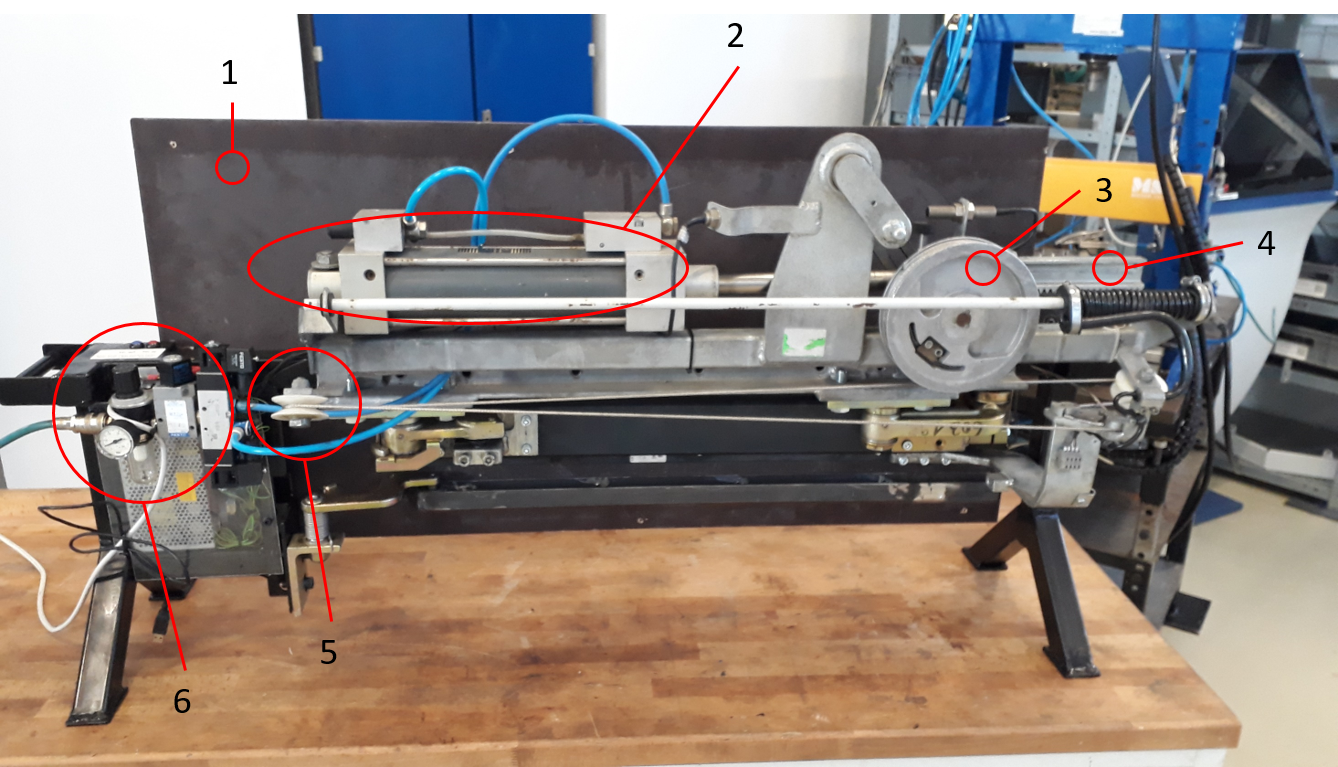
\includegraphics[width=\textwidth]{Foto_Türschließanlage_beschriftet.png}
	\caption{Ausgebaute Türschließanlage eines Zuges der Intercity-Klasse (Deutsche Bahn)\\1 Türattrappe, 2 Pneumatikzylinder, 3 Seilzugrad, 4 Zahnstange, 5 Seilrolle, 6 Pneumatikanschluss}
	\label{fig:foto_tureschliessanlage}
\end{figure}

Wartungen der Anlage werden im Rahmen einer präventiven Instandhaltung durchgeführt. Zu diesem Zweck werden auch die Seilrollen regelmäßig ausgetauscht. Die Instandhaltungsmaßnahme wird entweder nach sechs Jahren oder nach \num{1.2} Millionen gefahrenen Kilometern durchgeführt~\cite{db.2021}.

Die Seilrollen aus Kunststoff sind ohne Wälzlager auf Bolzen montiert. Verschleiß und Materialermüdung sind in erster Linie an der Mantelfläche der Bohrung zu erwarten, an der die Rolle auf dem Bolzen aufliegt. Fortschreitende Rissbildung aufgrund von Materialermüdung bestimmt die Lebensdauer der Seilrollen. Mit steigendem Grad der Beschädigung steigt auch das Risiko eines Gewaltbruchs durch Überlast. In diesem Fall fällt die Türschließanlage aus und eine nicht planmäßige Instandsetzungsmaßnahme ist erforderlich.

Kann zu einem beliebigen Zeitpunkt der Zustand der Seilrollen bestimmt werden, so kann jederzeit der Bedarf einer Instandhaltungsmaßnahme eingeschätzt werden. Unerwartete Ausfällen können so vermieden werden (vgl. \cref{ch:instandhaltungsstrategien}). Kann der aktuelle Zustand darüberhinaus mit einem zu erwartendem Änderungsverlauf in Zusammenhang gebracht werden, kann sogar eine Vorhersage zum Ausfallzeitpunkt abgegeben werden. Die Vorteile einer prädiktiven Instandhaltung können so genutzt werden (vgl.~\cref{sec:praediktive_instandhaltung})

Die Instandhaltung der Seilrollen kann durch einem PdM-Ansatz gelöst werden. Voraussetzung dafür ist Erstens, dass Messwerte vorliegen, die Informationen über den Zustand der Seilrolle beinhalten. Zweitens sind diese Informationen in ein Entscheidungsmodel zu integrieren, das anhand von neuen Messwerten den Zustand der Rollen bestimmen kann. Drittens muss eine Infrastruktur geschaffen werden mit der in festgelegten Zeitabständen aktuelle Messwerte aufgenommen und verarbeitet werden können.
%===============================================================================
\section{Erfolgskriterien}
\label{sec:erfolgskriterien_usecase}
Um bestimmen zu können ob die Umstellung der Instandhaltung auf einen PdM-Ansatz sinnvoll ist, muss eine ausgiebige Nutzwertanalyse abgeschlossen und mit dem aktuell verwendetem Instandhaltungsansatz verglichen werden. 

Aufgrund der prinzipiell verschiedenen Natur von CM, PM und PdM, lassen sich nur wenige Vergleichende kriterien bestimmen. Beispielsweise kann die Anzahl vermeidbarer Ausfälle nicht verglichen werden, weil bei einem PM-Ansatz dazu keine Informationen zur Verfügung stehen. (Für die modelbewertung in \cref{ch:modelbewertung} entspricht eine beschädigte Seilrolle der Kategorie 1; ein nicht vermeidbarer Ausfall entspricht demnach einer \textit{falsch negativen} Vorhersage.) Auch werden bei PM per Definition keine unnötigen Inspektionen durchgeführt, wie es bei PdM für falsch positive Meldungen der Fall wäre. Um einen Vergleich der beiden Ansätze erheben zu können, sind also allgemeinere vergleichende Kriterien zu finden.

Im Rahmen dieser Arbeit wird ausschließlich auf Kriterien eingegangen, die den Nutzwert des vorgeschlagenen PdM-Ansatzes quantifizieren. Die Kriterien werden für die Bewertung der maschinellen Lernmodelle herangezogen, die in \cref{sec:modellierung} erstellt werden. Die folgenden Kriterien definieren den Nutzen der PdM-Anwendung.

\textbf{Komplexität}\\
Idealerweise soll das Modell nicht nur möglichst korrekte Vorhersagen über den Zustand der Seilrollen abgeben können, sondern auch Informationen extrahieren, die für Verbesserungen der Konstruktion verwendet werden können. Dafür ist ein Model nötig dessen Entscheidungverfahren nachvollziehbar ist. Ein zu komplexes Model kann nicht unter praktikablen Bedingungen ausgewertet werden. Aus diesem Grund ist ein einfach nachzuvollziehendes Model einem komplexeren vorzuziehen.

\textbf{Qualität der Vorhersagen}\\
Damit der Usecase einen Mehrwert gegenüber dem vorherigen Vorgehen bietet, müssen die Vorhersagen des Models ein Mindestmaß an Genauigkeit bieten können. Die Zahl falsch positiver, wie auch falsch negativer Vorhersagen (Fehlalarme bzw. unentdeckte Beschädigungen), sollten möglichst gering ausfallen. Ein Mindestmaß für beide Eigenschaften hängt von der Qualität des gegenüber stehenden PM-Usecases ab. Weil -- wie einleitend erwähnt -- dieses Kriterium keinen direkten Vergleich zwischen dem PM- und PdM-Ansatz zulässt, werden Annahmen für die Mindestmaße getroffen (s.~\cref{sec:bewertungskriterien}).

Bei der Qualität der Vorhersagen sind falsch positive Vorhersagen geringer zu wichten als falsch negative. Falsch positive Vorhersagen haben eine unnötige Inspektion oder Austausch der Komponente zufolge, wohingegen falsch negative Vorhersagen zu einem unerwarteten Ausfall führen. Im ersten Fall entstehen Kosten durch Verschwendung; im zweiten durch die notwendige Behebung einer Störung. Letzteres ist jedoch in der Regel mit höheren Kosten verbunden. Deswegen wird falsch negativen Vorhersagen ein höheres Gewicht zugeschrieben als falsch positiven Vorhersagen (s.~\cref{tab:paarvergleich}). Das Kriterium lässt sich in Form der Sensitivität und Relevanz direkt auf die Bewertung des verwendeten Vorhersagemodelle anwenden.
%===============================================================================
\section{Einordnung in den Kontext der Bahntechnik}
\label{sec:kontext_bahntechnik_von_usecase}
Der eröffnete Usecase beruht auf allgemeinen Prinzipien von PdM. Darüberhinaus gehend ist es sinnvoll den Usecase in den Kontext der praktischen Bahntechnik ein zu ordnen. Insbesondere eine Diskusion über den tatsächlichen Bedarf, als auch eine Darstellungen des angewandten Wartungsvorgehen ist für eine Bewertung des Usecases zuträglich.

Um den Usecase in den Kontext der Bahntechnik zu stellen, wurden zwei Interviews mit Sachverständigen der Deutschen Bahn und der Hochbahn Hamburg geführt. Die folgenden Abschnitte geben die wichtigsten Ergebnisse dieser Interviews wieder.
%===============================================================================
\subsection{Interview: Hochbahn Hamburg}
\label{subsec:interview_hochbahn}
\textit{Interview mit Jürgen Beck~\cite{hochbahn.2020} am {23.11.2020}}

Herr Beck benannte im Allgemeinen Lager als Komponenten, deren Wartungen von Kenntnissen über den aktuellen Zustand profitieren kann. Sie gehören zu den Komponenten, die dem größten Verschleiß unterworfen sind und daher häufig zu ersetzen sind. Die Seilrollen sind nicht in Verbindung mit einem Wälzlager montiert, sondern stützen sich direkt auf einem Bolzen ab. Verschleiß -- bedingt durch Relativbewegung zwischen Bolzen und Rolle -- tritt also an der Seilrolle selbst auf. Vor diesem Hintergrund ist die Wahl, die Seilrollen mit einem PdM-Ansatz instand zu halten, ebenso sinnvoll wie für Wälzlager.

Bezogen auf den Betrieb der Hochbahn in Hamburg wurde diskutiert welche Auswirkungen ein Ausfall der Türschließanlage hat und ob sich daraus ein Bedarf für den vorgeschlagenen Usecase ableiten lässt. Herr Beck betonte, dass eine Störung der Türanlage nur in Ausnahmefällen einen bedeutsamen Einfluss auf den Betriebsablauf hat. Für einen solchen Ausnahmefall müssten mehrere Türschließanlage an dem selben Waggon ausfallen und der Waggon dürfte nicht durch Zwischentüren mit den anhängenden Waggons verbunden sein. Nur in einem solchen Fall ist ein sicherer Betrieb des Waggons nicht mehr möglich, weil Fluchtmöglichkeiten unzulässig beschränkt sind. Es wird nicht erwartet, dass eine derartiger Ausnahmefall eine Umstellung der Instandhaltung auf einen PdM-Ansatz rechtfertigen kann. Dies ist der auch der Grund dafür warum die Hochbahn Hamburg aktuell nicht an der Umsetzung einer PdM-Anwendung arbeitet, wie sie zu Beginn dieses Kapitels vorgeschlagen wurde.
%===============================================================================
\subsection{Interview: Deutsche Bahn}
\label{subsec:interview_deutsche_bahn}
\textit{Interview mit Dr. Jörg Lehmann~\cite{db.2021} am {27.01.2021}}

Herr Lehmann beschrieb das Vorgehen der Deutschen Bahn bei der Instandhaltung von Regional- und Fernverkehrszügen wie folgt: Unterschieden wird zwischen der \textit{betriebsnahen} und der \textit{schweren} Instandhaltung. Die betriebsnahe Instandhaltung wird durch den Zugbetreiber durchgeführt und umfasst Instandhaltungsmaßnahmen, die die kurzfristige Verfügbarkeit des Zuges gewährleisten. Im Gegensatz zur schweren Instandhaltung, wird sie nach Bedarf durchgeführt. Neben Reinigungsarbeiten und Reparaturen an Interiör, umfasst sie auch Arbeiten an technischen Systemen des Zuges. Eine Türstörung kann laut Lehmann in der Regel im Rahmen einer betriebsnahen Instandhaltung behoben werden. Das bedeutet, dass Maßnahmen zur vorausschauenden Instandhaltung kurzfristig umgesetzt werden können, ohne dafür neue Strukturen schaffen zu müssen.

Die schwere Instandhaltung wird entweder nach sechs Jahren Betriebsdauer oder nach \num{1.2} Millionen gefahrenen Kilometern vorgenommen. Sofern die festgelegte Kilometeranzahl noch nicht erreicht ist, kann nach einer Einschätzung durch Sachverständige, das Intervall	auf \num{8} Jahre angehoben werden. Zu Beginn der schweren Instandhaltung wird eine Eingangsuntersuchung vorgenommen. Daran schließen sich Instandhaltungsmaßnahmen in Form von Plan-, Sicherheits- und Außerplanarbeiten an. Planarbeiten stehen bereits im Vorfeld der schweren Instandhaltung fest und werden grundsätzlich durchgeführt. Sicherheitsarbeiten werden umgesetzt, ohne dass es dafür einer extra Auftragsstellung bedarf. Außerplanarbeiten bedürfen hingegen einer nachträglichen Auftragsstellung. Die Auftragsstellungen erfolgen auf Basis der Ergebnisse der Eingangsuntersuchung. Gegeben dem Fall, dass durch die PdM-Anwendung Informationen über den Zustand der Seilrollen vorliegen, kann ihre Instandhaltung im Rahmen von Planarbeiten erledigt werden. Es wird also ein Zeitvorsprung gewonnen, der eine Planung ermöglicht.

Die Aussagen von Herrn Beck bezüglich des Bedarfs des Usecases teilt Herr Lehmann. Auch seiner Ansicht nach ist der Einfluss einer Türstörung auf den Betriebsablauf klein, weswegen wirtschaftlicher Mehrwert nicht zu erwarten sei.
%===============================================================================


\cleardoublepage	
% \chapter{Methodik}
\label{ch:methodik}
Um eine zustandsbasierte -- und darauf aufbauend eine prädiktive -- Instandhaltung umsetzten zu können, ist es nötig Daten zu gewinnen, die diesen Zustand beschreiben, und ein Model zu erstellen, das diese auswertet. Es folgt eine Beschreibung der Methodik nach der die Ergebnisse aus \cref{ch:modelbewertung} erarbeitet werden. Die Methodik beschränkt sich auf die Entwicklung eines zustandbestimmenden Models.
%===============================================================================
\section{Versuchsaufbau}
\label{sec:versuchsaufbau}
\begin{wrapfigure}{r}{0.5\textwidth}
	\centering
	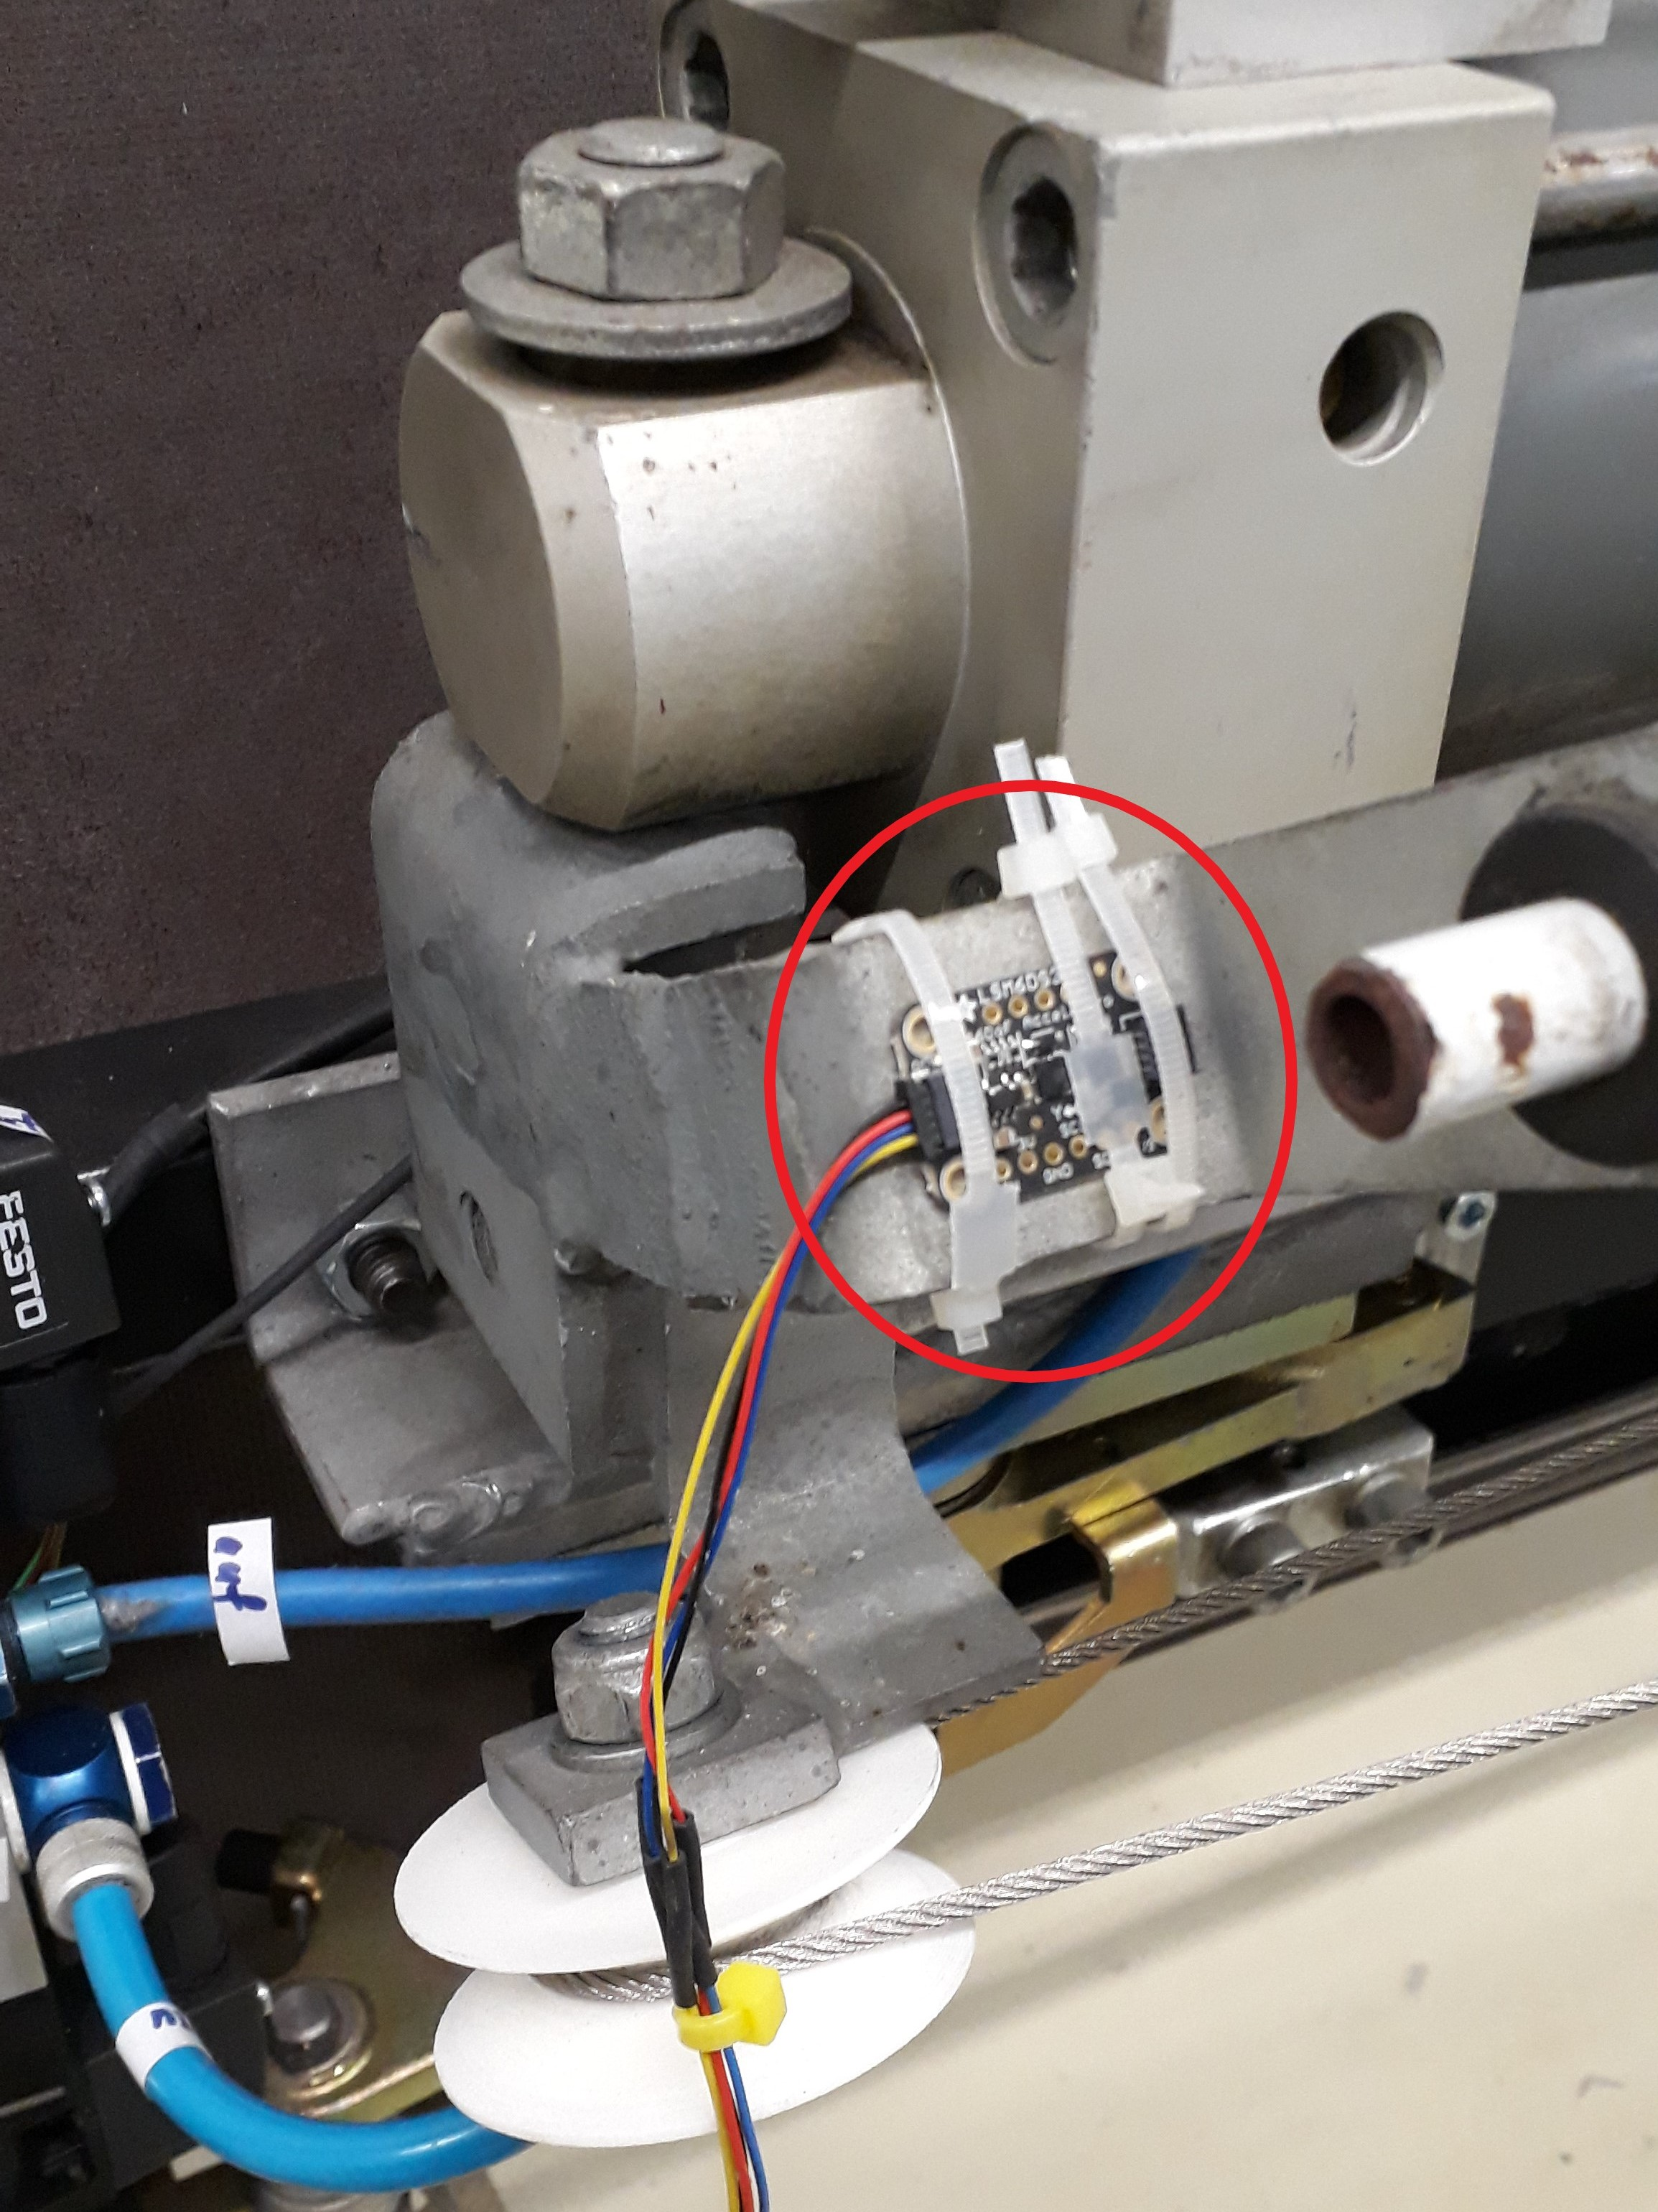
\includegraphics[width=6cm]{sensor.jpg}
	\caption{An Türschließanlage befestigter Beschleunigungssensor}
	\label{fig:beschleunigungssensor}
\end{wrapfigure}

Der in \cref{sec:messdaten} beschriebene Datensatz wird mit folgendem Messaufbau erfasst:

An die Türschließanlage ist eine Druckluftzufuhr (s.~\cref{fig:foto_tureschliessanlage} Pos.~6) angeschlossen, welche die Energie zum Antrieb des Kolbens liefert. Ein Druckregeler regelt den Luftdruck auf ca. \SI{550000}{\pascal} (\SI{80}{psi}). Der Luftstrom wird durch ein 5/2-Wegeventil (Model: VUVS-LK25-B52-D-G14-1B2-S; Fa. Festo) gesteuert, dass magnetisch betätigt wird. Die Ventilstellung bestimmt die Bewegungsrichtung des Kolbens. Zwischen Druckregeler und Wegeventil ist außerdem ein Absperrventil (MFH-3-1/8; Fa. Festo) verbaut. Dieses wird ebenfalls durch einen Elektromagneten betätigt und kappt die Luftzufuhr, wenn das System zum Stillstand gebracht werden soll.

Sämtliche Ventile werden über Relais mit den jeweils nötigen elektrischen Spannungen (\SI{24}{\volt}) versorgt. Die Schaltung der Relais -- und damit die Steuerung der Türschließanlage -- erfolgt durch einen Mikrocontroller vom Typ Arduino Uno (Fa. Az-Delivery). Dieser führt den Programmcode (Datei \enquote{csvwriter.ino}; s. Anhang) zur Versuchsdurchführung aus.  Dazu gehört auch das Auslesen des installierten Beschleunigungssensor und Gyroskops (s.~\cref{fig:beschleunigungssensor}). 

Die Position des Beschleunigungssensors ist so gewählt, dass keine konstruktive Änderung an der Türschließanlage vorgenommen werden muss. Abhängig von der Position des Sensors relativ zur Seilrolle sind unterschiedliche Messwerte zu erwarten. Da die absoluten Messwerte für die Klassifikation nicht von Bedeutung sind; sondern nur deren Unterschied in Bezug auf die Kategorien; erweist sich die Position des Sensors als geeignet.

Zur Speicherung der Daten werden diese über eine serielle USB-Schnittstelle an ein angeschlossenes Computersystem übertragen. Der dort, parallel laufende Programmcode (Datei: \enquote{csvwriter.py};s. Anhang) decodiert das Signal des Mikrocontrollers und speichert die Daten in einer passend formatierten CSV-Datei ab.

Um vergleichbare Datenpunkte zu erhalten wird für die Messreihe nicht das Original der Seilrolle verwendet, sondern mit im Lasersinterverfahren hergestellten Nachbildungen (s.~\cref{fig:seilrolle_isometrisch}). Die Festigkeit des Materials ist für den Versuch ausreichend. Nach dem Versuch wurden bei einer Sichtprüfung keine plastischen Verformungen festgestellt. Eine der Nachbildungen wurde mit Rillen versehen, die längst der Bohrung verlaufen (s.~\cref{fig:seilrolle_rillen}). Die Rillen simulieren Materialausbrüche als Folge von Pittings. Insgesamt weist die so künstlich beschädigte Seilrolle drei Rillen auf die um jeweils 45° zueinander verschoben sind.

\begin{figure}[ht]
	\centering
	\subfloat[Unbeschädigte Nachbildung der Seilrolle\label{fig:seilrolle_isometrisch}]{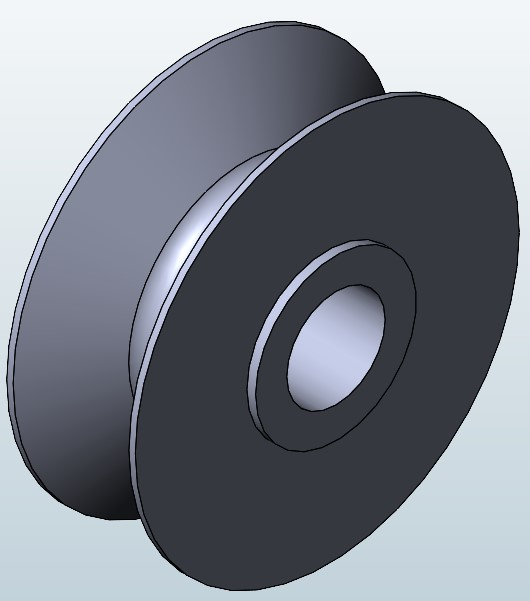
\includegraphics[width=0.35\textwidth]{seilrolle_isometrisch.jpg}}
	\qquad
	\subfloat[Rillen in künstlich beschädigten Nachbildung\label{fig:seilrolle_rillen}]{\includegraphics[width=0.43\textwidth]{seilrolle_rillen_bemaßt.jpg}}
	\caption{Nachbildungen der Seilrolle}
	\label{fig:cad_seilrolle}
\end{figure}

Mit verbauter intakter bzw. beschädigter Seilrolle werden jeweils 100 Datenpunkte aufgezeichnet. Ein Datenpunkt entspricht einem Öffnungs- und Schließvorgang, wie er durch den Programmcode vorgegeben wird.
%===============================================================================
\section{Messwerte und Datenaufbereitung}
\label{sec:messdaten}
Der Datensatz weißt \num{1441} Merkmale auf. Je \num{240} davon bilden eine Zeitreihe einer der Messwerte von Beschleunigungssensor bzw. dem Gyroskop. Insgesamt beinhaltet der Datensatz folgende Messwerte (Achsenrichtungen beziehen sich auf den Beschleunigungssensor):
\begin{itemize}
	\item Beschleunigung aller drei Raumachsen
	\item Rotationgeschwindigkeiten um alle drei Raumachsen
	\item Zykluszeit: Dauer eines Öffnungs- und Schließvorgangs (inkl. Laufzeitpause das Programmcodes)
\end{itemize}

Die Messgrößen der Beschleunigungen und der Rotationgeschwindigkeiten wurden ausgewählt, da sie das Schwingungsprofil der Anlage beschreiben. Es wird erwartet, dass sich dieses mit dem Grad der Beschädigung der Seilrollen ändert. Es kann also erwartet werden, dass die gewählten Messgrößen aussagekräftig über den Zustand der Seilrollen sind. Voraussetzung ist das, dass eine andere Ursache für die Änderung des Vibrationsprofils nicht in Frage kommt. Diese Voraussetzung ist hier geben, weil die Seilrolle die einzige Variable im Versuchsaufbau ist.

Für die Modelentwicklung ist es sinnvoll die Rohdaten in einem beschreibenden Datensatz zusammen zu fassen. Die erstellten Modelle basieren auf Entscheidungsbäumen mit maximal sechs Ebenen (vgl. \cref{sec:modelauswahl} bzw. \cref{sec:modellierung}). Das bedeutet, dass jeder Entscheidungsbaum nur einen sehr kleinen Anteil der Merkmale des Rohdatensatzes verwenden kann. Dies kann eine ungewünschte negative Auswirkung auf die Entwicklung des Models haben. Es besteht die Möglichkeit, dass ein Model nur Merkmale berücksichtigt, die zu dem selben Messwert gehören, weil diese zufällig eine höhe Aussagekraft für die Zuordnung der richtigen Kategorien haben, aber nicht zwangsläufig für die Population gültig sind. Informationsgehalt der anderen Messwerte geht so verloren. Mit einem Datensatz, der die Informationen der Zeitreihen in statistischen Parametern zusammenfasst, kann eine größerer Anteil dieser Merkmale verwendet werden und so mehr Informationen des Rohdatensatzes genutzt werden. Die Entscheidungsbäume der erstellten Modelle besitzen maximal \num{32} Knoten (s.~\cref{sec:modellierung}). Sie können alle Merkmale des beschreibenden Datensatzes nutzen, der insgesamt über \num{25} Merkmale verfügt.

Aus dem genannten Grund wird ein beschreibender Datensatz aus den Rohdaten abgeleitet. Der Datensatz beschreibt die Messungen anhand folgender Parameter (ersten vier je Messgröße).
\begin{itemize}
	\item Minimalwert
	\item Maximalwert
	\item Median
	\item Standardabweichung
	\item Zykluszeit
\end{itemize}
%===============================================================================
\section{Modelauswahl}
\label{sec:modelauswahl}
Die Menge an Klassifikationsmodelle ist größer als sie im Rahmen dieser Arbeit berücksichtigt werden kann. Jedoch kann eine sinnvolle Vorauswahl an geeigneten Modeltypen getroffen werden. So kann die Anzahl der Modelle, die tatsächlich entwickelt und verglichen werden müssen, auf ein handhabbares Maß reduziert werden.

Die Vorauswahl geeigneter Modeltypen richtet sich nach folgenden Anforderungen. Die Anforderungen sind von den Erfolgskriterien Komplexität und Modelqualität des Usecases abgeleitet (vgl.~\cref{sec:erfolgskriterien_usecase}).

\begin{itemize}
    \item Für den vorhandenen Datensatz muss eine hohe Modelqualität erwartet werden können. Die Modelqualität wird für den Usecase durch die Sensitivität und Relevanz der Klassifikation bestimmt.
    \item Das Model muss prinzipiell nachvollziehbar sein. D.h. es muss möglich sein die Ergebnisse des Modell auf Logikfehler hin untersuchen zu können, um zufällige Abweichungen der Ergebnisse identifizieren zu können. Gleichzeitig muss die Komplexität quantifizierbar sein, damit ein Vergleich möglich ist.
\end{itemize}

Unter den genannten Voraussetzungen kommen diese Modeltypen in Frage:
\begin{itemize}
    \item Logistic Regression
    \item Entscheidungsbäume
    \item k-nearest neighbors
    \item Naive Bayes
\end{itemize}

Modeltypen, die von ihrem Funktionsprinzip her keine Beurteilung des Entscheidungsprozesses zulassen, sind erfüllen die Grundvorsetzung für das Komplexitäts-Kriterium nicht. \textit{Support Vector Machines} und \textit{neuronale Netze} scheiden daher aus.

Für die Modelentwicklung werden nur Modelle verwendet, die auf Entscheidungsbäumen basieren. Diese Modeltypen sind günstig zu visualisieren; und damit nachvollziehbar; und lassen auf dicht besetzten Datensätzen (vgl.~\cref{sec:messdaten}) gute Modelqualitäten erwarten. Außerdem ist eine weniger aufwendige Aufbereitung der Daten nötig, weil die Daten nicht skaliert werden müssen~\cite[S.~84--85]{Muller.2017}

Die Modelentwicklung wird; auf die Vorauswahl hin; weiter auf drei Algorithmen beschränkt:
\begin{itemize}
    \item einfacher Entscheidungsbaum
    \item Random Forest
    \item Gradient Boosted Trees
\end{itemize}
%===============================================================================
\section{Bewertungskriterien}
\label{sec:bewertungskriterien}
Aus der Vorauswahl an Algorithmen soll das Model bestimmt werden, das die Anforderungen an den Usecase (s.~\cref{sec:erfolgskriterien_usecase}) bestmöglich erfüllt. Es ist deswegen notwendig den Erfüllungsgrad der Anforderungen durch die einzelnen Modelle quantifizieren zu können. Die Bewertung der Modelle erfolgt in zwei Schritten.

Erstens werden Bewertungskriterien definiert, die verschiedenen Modeleigenschaften einen konkreten Wert zwischen \num{0} und \num{1} zuweisen. Im zweiten Schritt werden die Bewertungskriterien zu einer Präferenzfunktion zusammengefasst. Die Präferenzfunktion addiert die gewichteten Kriterienwerte auf. So wird für ein Model ein Gesamtscore ermittelt, der ebenfalls Werte zwischen \num{0} und \num{1} annehmen kann. Ein Wert von \num{1} entspricht einer idealen Erfüllung der Anforderungen; \num{0} spricht für ein völlig ungeeignetes Model.

\cref{tab:bewertungskriterien_fuer_praeferenzfunktion} zeigt die Bewertungskriterien und die zugeordneten Kriterienwerte. Die Gewichtungen der Kriterien wurden durch einen Paarvergleich bestimmt; siehe \cref{tab:paarvergleich}. Eine \num{1} bedeutet dabei, dass das Kriterium weniger wichtig ist; eine \num{2}, dass es wichtiger ist als das Vergleichskriterium.

\begin{table}[ht]
	\begin{tabularx}{\textwidth}{|p{2.5cm}|p{2.5cm}|c|X|}
		\hline
		\rowcolor{lightgray}
		Kriterium & Wertezuordnung & Gewichtung & Bemerkungen \\ 
		\hline
		\multirow[t]{9}{*}{Baumtiefe (Komplexität)} & \multirow[t]{9}{*}{\makecell{$\num{1} \rightarrow \num{1}$\\adsfadf\\asdfadf\\asdf}} & \multirow[t]{9}{*}{\num{0.165}} & \multirow[t]{9}{*}{Insgesamt wird die Komplexität mit \num{0,22} gewichtet. Da die Komplexität exponentiell mit der Baumtiefe steigt und linear mit der Baumanzahl wurde entschieden, dass die Baumtiefe \SI{75}{\percent} der Komplexität ausmacht; also $0.22\cdot0.75=0,165$. Die restlichen \SI{0.055}{\percent} entfälle auf die Baumanzahl}\\
		% & $\num{2} \rightarrow \num{0,75}$ &&\\
		% & $\num{3} \rightarrow \num{0,5}$&&\\
		% & $\num{4} \rightarrow \num{0,25}$&&\\
		% & $>=5 \rightarrow \num{0}$&&\\
		\hline
		% \multirow{5}{2.5cm}{Baumanzahl (Komplexität)} & \multirow{5}{*}{$\begin{array}{ll}
		% 	\num{1} \mathrm{bis}19 & \rightarrow \num{1}\\
		% 	\num{20}\mathrm{bis}39 & \rightarrow \num{0,75}\\
		% 	\num{40}\mathrm{bis}59 & \rightarrow \num{0,5}\\
		% 	\num{60}\mathrm{bis}79 & \rightarrow \num{0,25}\\
		% 	>=80 & \rightarrow \num{0}\\
		% \end{array}$} & \multirow{5}{*}{\num{0.055}} & s. Baumtiefe\\
		% \multirow{5}{*}{Baumanzahl (Komplexität)} & \multirow{5}{*}{$\begin{array}{ll}
		% 	
		% \end{array}$} \num{1} $\rightarrow$ \num{1} & \multirow{5}{*}{\num{0.055}} & s. Baumtiefe\\ 
		% & \num{2} $\rightarrow$ \num{0,75} &&\\
		% & \num{3} $\rightarrow$ \num{0,5} &&\\
		% & \num{4} $\rightarrow$ \num{0,25} &&\\
		% & $>=5$ $\rightarrow$ \num{0} &&\\
		% \hline
		% \multirow{5}{*}{Sensitivität} & \multirow{5}{*}{\thead{1,0 $\rightarrow$ 1\\sadfdsafsadf\\afdsdsaf\\sadfsadf}} & \multirow{5}{*}{\num{0.44}} & Je höher die Sensitivität ist, desto weniger falsch negative Vorhersagen werden getroffen. Für den PDM-Usecase bedeutet es, dass mehr Instandhaltungsarbeiten geplant werden können. \\
		% \hline
        % \multirow{5}{*}{Relevanz} & xx & \num{0.33} & Eine hohe Relevanz bedeutet, dass wenige falsch positive Vorhersagen getroffen werden. Entsprechend niedrig fällt die Anzahl unnötiger Inspektionen für den PDM-Usecase aus.\\
		\hline
		\caption{Bewertungskriterien für Präferenzfunktion}%muss unten sein, sonst caption über Tab
		\label{tab:bewertungskriterien_fuer_praeferenzfunktion}	%zum referenzieren
	\end{tabularx}
\end{table}

Die Komplexität bezieht sich auf die Anforderung, dass das Model nachvollziehbar sein muss. Für die Komplexität gilt, dass sie so gering wie möglich sein sollte. Quantifiziert wird die Komplexität durch die Anzahl der Baumebenen (Tiefe) und die Anzahl der Bäume, die zusammen ein Model bilden.

Die Sensitivität beschreibt wie viele Datenpunkte mit positiver Kategorie als solche erkannt werden. Im Kontext der vorausschauende Instandhaltung bedeutet die Sensitivität welcher Anteil an bevorstehenden Ausfällen vermieden werden kann. Ihr Betrag sollte also möglichst groß sein. Es wird die Bedingung gestellt, dass mindestens \SI{95}{\percent} aller Ausfälle richtig vorhergesagt werden müssen, damit ein Wert von \num{1} vergeben wird.

Die Relevanz beschreibt wie viele Datenpunkte tatsächlich der positiven Kategorie angehören von denen, die als solche eingestuft worden sind. Eine niedrige Relevanz bedeutet demnach eine große Anzahl Fehlalarme. Da Fehlalarme jedoch verhältnismäßig kleine Kosten -- im Vergleich zu ungeplanten Ausfällen -- nach sich ziehen, kann auch eine niedrige Relevanz toleriert werden.

\begin{table}[h]
	\begin{tabularx}{\textwidth}{|l|ccc|c|r|}
		\hline
		& \rotatebox{90}{Komplexität} & \rotatebox{90}{Sensitivität} & \rotatebox{90}{Relevanz} & \rotatebox{90}{Summe} & Gewicht\\
		\hline
		Komplexität & -- & 1 & 1 & 2 & 0,22\\
		Sensitivität & 2 & -- & 2 & 4 & 0,44\\
		Relevanz & 2 & 1 & -- & 3 & 0,33\\
		\hline
		\hline
		Gesamt & \multicolumn{2}{c}{} & & 9 & $\approx$ 1\\
		\hline
		\caption{Paarvergleich zur Bestimmung der Gewichtungen der Bewertungskriterien}
		\label{tab:paarvergleich}
	\end{tabularx}
\end{table}

Mit den Werten aus \cref{tab:bewertungskriterien_fuer_praeferenzfunktion} wird die Präferenzfunktion aufgestellt:

\begin{equation*}
	\text{Gesamtscore}=0.165\cdot t+
	0.055\cdot a+0.44\cdot s+0.33\cdot r
	\label{eq:praeferenzfunktion}
\end{equation*}

Dabei ist $t$ der Wert, der dem Bewertungskriterium \textit{Tiefe} zugeordnet wird. Entsprechend ist $a$ der Wert zur Baumanzahl, $s$ der Wert zur Sensitivität und $r$ der Wert zur Relevanz (vgl. \cref{tab:bewertungskriterien_fuer_praeferenzfunktion}).
%===============================================================================
\section{Modellierung}
\label{sec:modellierung}
Im Vorfeld der Modellierung wird der Datensatz in Trainings- und Testdaten aufgeteilt. Der Trainingsdatensatz enthält \SI{75}{\percent}, der Testdatensatz \SI{25}{\percent} der Daten. 

Für die Modellierung der gewählten Algorithmen (s.~\cref{sec:modelauswahl}) wird jeweils auf gleiche Weise verfahren. Damit ein Vergleich zwischen den verschiedenen Modeltypen sinnvoll ist, müssen alle für die gegebene Anwendung optimiert werden. Zunächst wird für jedes Model ein Parametergitter definiert, aus dem die idealen Parameter bestimmt werden. Für die unterschiedlichen Modeltypen beinhalten die Parametergitter auch unterschiedliche Parameter (s. Anhang und vgl. \cref{sec:einfache_entscheidungsbaeume}--\cref{sec:gradient_boosted_trees}), damit jedes Model entsprechend seinem Typ optimiert werden kann. Die Parameter \textit{maximale Baumtiefe} und \textit{Baumanzahl} haben aber alle Parametergitter gemein. Für jede Parameterkombination wird ein Model erstellt. Diese werden verglichen und so die ideale Parameterkombination bestimmt (\textit{Gittersuche}). Mit den Ergebnissen der jeweils ersten Gittersuche wird das Parametergitter verfeinert und die Gittersuche erneut ausgeführt.

Die Modelle, die im Laufe der Gittersuche erstellt werden, werden mit einer 10-fachen Kreuzvalidierung ausgewertet und der Vergleich der Modelle erfolgt währenddessen anhand der erreichten Sensitivität. Nach \cref{sec:bewertungskriterien} fällt der Sensitivität nämlich die größte Gewichtung für die Modellbewertung zu.

Der Aufbau von Entscheidungsbäumen ist von Pseudo-Zufallszahlen abhängig. Um reproduzierbare Modelle zu entwickeln, wird für die Generierung dieser Zahlen ein Startwert von \num{42} verwendet. Allen Modelinstanzen wird dieser Wert als Parameter übergeben.

Während der Parameterstudie des GBT wurde Overfitting des Models vermutet, da die Sensitivität bei einem Wert von \num{1} lag und die Baumanzahl mit \num{95} deutlich größer war als die des Random Forest (19). Um dem entgegen zu wirken, wurde für den GBT im Anschluss an die ursprüngliche Gittersuche die Baumanzahl soweit reduziert bis ein realistischer Sensitivitätswert vorlag.
%===============================================================================\cleardoublepage
% \chapter{Modelbewertung und Diskussion}
\label{ch:modelbewertung}
WAS SIND DIE ERGEBNISSE DER MODELLIERUNG? WIE ERFÜLLEN DIE MODELLE DIE BEWERTUNGSKRITERIEN? WELCHES MODEL IST AM BESTEN FÜR DEN USECASE GEEIGNET UND WARUM? WIE SIND DIE ERGEBNISSE DER MODELLE ZU INTERPRETIEREN? WELCHE SCHWACHSTELLEN BIETET DIE GEWÄHLTE BETRACHTUNG?

\cref{tab:metrikwerte_der_trainierten_modelle} zeigt die Parameter der besten Modelle jedes Typs und deren Sensitivität und Relevanz. Zusätzlich ist der Gesamtscore aufgeführt der sich aus der Präferenzfunktion ergibt.

\begin{table}[ht]
	\raggedright
	\begin{tabularx}{\textwidth}{ | l | r | r | r|}
		\hline
		\rowcolor{lightgray}
		Metrik & Baum & Random Forest & GBT\\
		\hline
		Tiefe & 1 & 1 & 1\\
		Anzahl Bäume & 1 & 19 & 26\\
		Sensitivität & \num{0.87} & \num{0.85} & \num{0.91}\\
		Relevanz & \num{0.91} & \num{0.85} & \num{0.91}\\
		\hline
		\hline
		Nutzen & \num{0.77} & \num{1} & \num{0.87}\\
		\hline
	\end{tabularx}
	\caption{Metrikwerte der trainierten Modelle und Nutzenwert nach Präferenzfunktion}%muss unten sein, sonst caption über Tab
	\label{tab:metrikwerte_der_trainierten_modelle}	%zum referenzieren
\end{table}


Den Ergebnissen nach ist das Random Forest Modell am besten geeignet, um für Vorhersagen zu dem Usecase verwendet zu werden. Nach \cref{tab:metriken_praeferenzfunktion} erreicht das Model für jedes Bewertungskriterium die maximale Punktzahl. Von allen Modellen weist es die höchste Sensitivität auf. Seine Relevanz ist zwar die niedrigste der dreien; den Kriterium wird nach \cref{tab:metriken_praeferenzfunktion} aber dennoch der gleiche Wert zugewiesen wie den anderen beiden Modellen.

Der Random Forest fällt auffällig simple aus. Die Tiefe der Bäume ist minimal und die Anzahl der Bäume ist klein. Üblicherweise zählt ein Random Forest hundert Bäume oder mehr. Die geringe Anzahl ist vermutlich auf den Datensatz zurückzuführen. Ein Hinweis darauf bietet die Tatsache, dass alle Modelle die minimale Baumtiefe verwenden und alle das Merkmal \enquote{gx\_median} verwenden. Zwar verwenden der Random Forest und die GBT einen groß Teil der Merkmale, jedoch erreicht selbst der einfache Entscheidungsbaum, der nur \enquote{gx\_median} verwendet, verhältnismäßig gut Ergebnisse. Daraus wird gefolgert, dass sich die Kategorien gut anhand dieses einen Merkmals einteilen lassen. Das erklärt die niedrige Komplexität des Random Forest.

\todo{Referenz für Diagramm einfügen} zeigt die Verteilung der \enquote{gx\_median}-Werte für die positive (beschädigt) wie für die negative Kategorie (intakt). Für die positive Kategorie zeigt sich annäherd eine Normalverteilung. Die negative Kategorie hingegen ist bimodal. Es wird daher vermutet, dass dieser Verteilung eine weitere nicht näher bekannte Kategorie zu grunde liegt.

Von der negativen Kategorie überlagert sich nur der linke Bereich mit den positiven Datenpunkten. Der Großteil der Datenpunkte lässt sich anhand des abgebildeten Merkmals richtig den beiden Kategorien zuordnen. Dies erklärt warum selbst die Qualität des einfachen Entscheidungsbaums -- gemessen an den Bewertungskriterien -- relativ hoch ist. Es macht auch deutlich warum alle Modelle Bäume mit je nur einem Knoten erstellt haben. In Kombination mit dem wichtigsten Merkmal liefern die übrigen Merkmale nur noch wenige Informationen und verzehren ggf. das Ergebnis nur. Andernfalls hätte der einfache Entscheidungsbaum davon profitieren können, mehrere Merkmale zu verwenden.

Damit ist auch begründet warum Random Forest und GBT ungewöhlich wenige Bäume aufweisen.\cleardoublepage
% \chapter{Zusammenfassung und Ausblick}
\label{ch:fazit}
Für Umlenkrollen einer Türschließanlage wurde ein Anwendungsfall für eine vorausschauende Wartung erdacht. Dazu wurden Kriterien erarbeitet, die es ermöglichen den Wert des Anwendungsfalls zu quantifizieren. Für den theoretischen Anwendungsfall wurden außerdem eine Einordnung in den Kontext praktischer Instandhaltungverfahren in der Bahntechnik und eine Bewertung des Bedarfs vorgenommen.

Um in die Problemstellung einzuführen wurden wichtige Grundlagen der vorausschauenden Instandhaltung beleuchtet, indem die Instandhaltung als solches, sowie verschiedene Instandhaltungsstrategien dargelegt wurden. Insbesondere wurde das Verbesserungspotential dargestellt, welche PdM gegenüber den anderen Instandhaltungsstrategien bietet.

Desweiteren wurden drei maschinelle Lernmodelle beschriebenen, die zur Lösung der Problemstellung herangezogen wurden. Die Wahl dieser drei Modeltypen wurde im weiteren Verlauf begründet. Die trainierten Modelle wurden im Rahmen einer Parameterstudie optimiert und bewertet, sodass ein Random Forest als das Model bestimmt werden konnte, das den Anforderungen an den PdM-Usecase am besten gerecht wird. Dabei ist zu beachten, dass das Model bislang nur zwischen zwei klar definierten Zuständen der Umlenkrolle unterscheiden kann. In aktuellen Stadium kann das Model zwar für eine zustandorientierte Wartung der Umlenkrollen dienen; es ist aber noch nicht für eine vorausschauende Instandhaltung im eigentlichen Sinne fähig. Dazu ist das Model auf weitere Beschädigungszustände zu erweitern und deren zugehörigen Betriebszeiten zu berücksichtigten.

Um die Modelle zu entwickeln wurden Messreihen aufgezeichnet, die das Vibrationsprofil der Türschließanlage beschreiben. Die Qualität der Modelle wurde durch Zusammenfassung der Rohdaten in einem beschreibenden Datensatz verbessert. Außerdem wurde festgestellt, dass das Merkmal \enquote{gx\_median} einen hohen Informationsgehalt bezüglich der Kategorien der Datenpunkte aufweist. Diese Erkenntnis ist voraussichtlich für eine detailliertere Analyse des mechanischen Systems Türschließanlage nützlich; ebenso wie für die Optimierung des Datensatzes.
%===============================================================================\cleardoublepage


% 							Backmatter
%================================================================
%Literatur
\printbibliography[heading=bibintoc]
\cleardoublepage

%Abkürzungs- und Symbolverzeichnis
\renewcommand{\chaptermark}[1]{\markboth{#1}{}}

\chapter*{Abkürzungs- und Symbolverzeichnis}
\addcontentsline{toc}{chapter}{Abkürzungs- und Symbolverzeichnis}
\label{symbole_abk}
\chaptermark{Abkürzungs- und Symbolverzeichnis}
%================================================================
\noindent 
\textit{Abkürzungen}
\par
\vspace{6pt}
\par
\noindent 
\begin{tabular}{@{}p{2cm}l}
	AC   & Air Compressor, Luftverdichter               \\
	APH  & Air Preheater, Luftvorwärmer                 \\
	CC   & Combustion Chamber, Brennkammer              \\
	EXP  & Expander                                     \\
	HRSG & Heat Recovery Steam Generator, Abhitzekessel
\end{tabular}
%================================================================
\vspace{18pt}	% <-- comment/uncomment if pagebreak is required
%\clearpage		
\par
\noindent 
\textit{Lateinische Symbole}
\par
\vspace{6pt}
\par
\noindent 
\begin{tabular}{@{}p{2cm}l}
	$c$       & Spezifische Kosten je Exergieeinheit, \euro/J\textsubscript{ex} \\
	$\dot C$  & Kostenstrom, \euro/h                                            \\
	$CC$      & Kapitalgebundene Kosten, \euro                                  \\
	$c\!f$    & Capacity Factor, Jährliche Auslastung, --                       \\
	$e$       & Spezifische Exergie, J/kg                                       \\
	$\bar{e}$ & Spezifisch molare Exergie, J/mol                                \\
	$\dot E$  & Exergiestrom, W                                                 \\
	$f$       & Exergoökonomischer Faktor, --                                   \\
	$fc$      & Spezifische Brennstoffkosten, \euro/J                           \\
	$FC$      & Brennstoffkosten, \euro                                         \\
	$h$       & Spezifische Enthalpie, J/kg                                     \\
	$\dot H$  & Enthalpiestrom, W                                               \\
	$HHV$     & Brennwert, J/kg
\end{tabular}
%================================================================
\vspace{18pt}	% <-- comment/uncomment if pagebreak is required
%\clearpage
\par
\noindent 
\textit{Griechische Symbole}
\par
\vspace{6pt}
\par
\noindent 
\begin{tabular}{@{}p{2cm}l}
	$\Delta$      & Differenz                      \\
	$\varepsilon$ & Exergetischer Wirkungsgrad, -- \\
	$\eta_s$      & Isentroper Wirkungsgrad, --    \\
	$\kappa$      & Isentropenexponenten, --       \\
	$\lambda$     & Luftzahl, --
\end{tabular}
%================================================================
%\vspace{18pt}	% <-- comment/uncomment if pagebreak is required
\clearpage
\par
\noindent 
\textit{Hoch- und tiefgestellte Indizes}
\par
\vspace{6pt}
\par
\noindent 
\begin{tabular}{@{}p{2cm}l}
	0   & Referenzpunkt, Thermodynamische Umgebung \\
	a   & Avarage, Mittlere                        \\
	D   & Destruction, Vernichtung                 \\
	F   & Fuel, Brennstoff, Aufwand                \\
	net & Netto
\end{tabular}
%================================================================
\cleardoublepage

%Abbildungsverzeichnis
\addcontentsline{toc}{chapter}{\listfigurename}
\listoffigures
\cleardoublepage

%Tabellenverzeichnis
\addcontentsline{toc}{chapter}{\listtablename}
\listoftables
\cleardoublepage

%Anhang
\appendix
% \part*{CD-Anhang}
% \addcontentsline{toc}{chapter}{Anhang}
\chapter*{Anhangsinhalt auf CD}
\begin{itemize}
    \item Rohdatensatz
    \item Programmcode zur Erstellung maschineller Lernmodelle
    \item nicht öffentliche Literatur
    \item Programmcode für Messversuch
    \item CAD-Datei Seilrollennachbildung
\end{itemize}
%================================================================
\end{document}

% ToDo

% Vorlage für Tabellenumgebung vorbereiten